\documentclass[prd, nofootinbib, floatfix, 11pt,tightenlines,times]{article}

% latex W13report.tex; bibtex W13report; latex W13report; latex W13report; dvips W13report; gv W13report.ps

\usepackage[paperwidth=8.5in,paperheight=11in,centering,margin=1in]{geometry}
\usepackage{amsmath}
\usepackage{amsbsy}
\usepackage{natbib}
\usepackage{rotating}
\input epsf
\usepackage{amsmath}
\usepackage{wasysym}
\usepackage{subfigure}
\usepackage{graphicx}
\usepackage{epsfig}
\usepackage{color}
%\usepackage{ulem}
%\usepackage{epstopdf}

\renewcommand{\thefootnote}{\fnsymbol{footnote}}

%\renewcommand{\baselinestretch}{0.98}
\usepackage{epsfig}
\usepackage{titletoc}

% HOW TO SET UP AN 8.5 x 11:
% http://www.pages.drexel.edu/~pyo22/students/latexRelated/latexTutorial.html
\topmargin -1.5cm        % read Lamport p.163
\oddsidemargin -0.04cm   % read Lamport p.163
\evensidemargin -0.04cm  % same as oddsidemargin but for left-hand pages
\textwidth 16.59cm
\textheight 21.94cm 
\parskip 7.2pt           % sets spacing between paragraphs
\parindent 0pt		     % sets leading space for paragraphs

\def\aap{{\it Astr.~Ap.}}     %Astronomy & Astrophysics%
\def\aaps{{\it A\&AS}}
\def\apj{{\it ApJ}}

\author{Andrew Becker, Simon Krughoff, Andrew Connolly, Russell Owen}
\title{Report on Late Winter2013 Production: Image Differencing}
\date{\today}

\begin{document}

\maketitle

We're done!

\clearpage
\tableofcontents
\clearpage

\section{Introduction}

The focus of this production is to optimize and quantify the false
positive rate in the Psf--matched subtraction of a science image and a
reference image (referred to as the template image below).  The metric
we optimize is the number of false detections that are detected and
measured on the image difference.  We calculate several additional
quality metrics during the image subtraction process, and correlate
them with the number of false detections, as a means to predict the
number of false detections we may expect downstream from the image
subtraction.

\subsection{Algorithm and Background {\bf ANDYB}}

We assume that science image $S(x,y)$ can be modeled as a convolution
of the template image $T(x,y)$ by a PSF--matching kernel $K(u,v,x,y)$.
We further assume that the kernel may be decomposed using a set of
basis functions $K(u,v) = \sum_i a_i K_i(u,v)$, where the coefficients
in front of each basis are determined through:
%
\begin{eqnarray}
C_i & \equiv & (K_i \otimes T) \\ \nonumber
b_{i}  & = & \sum_{x,y} {{C_i(x,y) S(x,y)}\over{\sigma^2(x,y)}}   \nonumber \\ 
M_{ij} & = & \sum_{x,y} {{C_i(x,y) C_j(x,y)}\over{\sigma^2(x,y)}}  \nonumber \\ 
a_{i}  & = & M^{-1}_{ij} b_{j} \nonumber 
\label{eq-soln}
\end{eqnarray}
where $\sigma^2(x,y)$ is the per--pixel variance stored in the {\tt
  variance} plane of each LSST {\tt exposure}.  To generate a
spatially varying model for the kernel, we assume that the relative
weights of the basis functions $a_i$ themselves vary spatially,
i.e. $K(u,v,x,y) = \sum_i a_i(x,y) K_i(u,v)$.  We also assume that
there is a differnetial background between the two images $b(x,y)$
that may be fit for using a low--order Chebyshev.  The image
difference is then calculated through $D(x,y) = S(x,y) - T(x,y)
\otimes K(u,v,x,y) - b(x,y)$.

The basis functions themselves $K_i(u,v)$ are a degree of freedom in
this problem.  The original implementations \citep{Alard98,Alard00}
used a set of 3 Gaussians (represented by our {\tt Config} variable
nGauss), each with a different sigma (sigGauss), and each modified by
a Laguerre polynomial to a given order (degGauss).  Subsequent studies
\citep[e.g.][]{2007AN....328...16I} have suggested that a constant
ratio be maintained between the different Gaussian widths, such that
$\sigma_{i+1} = \beta \times \sigma_{i}$.  We use the value $\beta =
2.0$ for this production.  We set the scale for sigma by noting that,
under the assumption that the Psfs of the images are Gaussian
($\sigma_S$ for the science image and $\sigma_T$ for the template
image), the sigma of the matching kernel should be simply $\sigma_K^2
= \sigma_S^2 - \sigma_T^2$.  We use this width for the central
Gaussian in our sequence, when we use more than one Gaussian, or the
sole Gaussian in the sequence when we use only one.

Detection on the difference image occurs through correlation of
$D(x,y)$ with the science image's Psf, yielding optimally filtered
detection image $D'(x,y) = D(x,y) \circ Psf_S(x,y,u,v)$ where $\circ$
denotes correlation.  The values of the pixels in $D'(x,y)$ provide a
maximum likelihood estimate of there being a point source at that
position.  Detection occurs by simply finding pixels that are more
than N sigma above the variance.  

In this production, we investigate two orders of operations for the
optimal filtering by the Psf.  In the first, we Psf--match the
template image to a pre--filtered science image:
\begin{eqnarray}
D_{Pre}(x,y) & = & S(x,y) \circ Psf_S(x,y,u,v) - T(x,y) \otimes K(u,v,x,y) \nonumber \\ 
D'_{Pre}(x,y) & = & D_{Pre}(x,y). \nonumber 
\end{eqnarray}
By pre--smoothing the image that we are matching the template to --
$S(x,y) \circ Psf_S(x,y,u,v)$ -- we more frequently avoid the case
of psf--matching {\it deconvolution}, where the FWHM of $T$ is
narrower than $S$.  This pre--filtering increases the FWHM of the
image by $\sqrt{2}$.  The Psf matching kernels will need to be
correspondingly larger to account for the larger Psfs.  We are able to
run detection directly on this image.

In the second, which is the classical implementation of the problem,
we create a difference image that is then post--filtered with the Psf
for detection:
\begin{eqnarray}
D_{Post}(x,y) & = & S(x,y) - T(x,y) \otimes K(u,v,x,y) \nonumber \\ 
D'_{Post}(x,y) & = & D_{Post}(x,y) \circ Psf_S(x,y,u,v).  \nonumber 
\end{eqnarray}

%One complication is that measurement on $D'_{Pre}$ is necessarily
%different than on $D'_{Post}$.

\subsection{Implementation {\bf ANDYB}}

We describe the general set of classes and algorithms that are used to
undertake these operations in the LSST DM stack.  We assume that we
have the science image $S(x,y)$ as a {\tt calexp} instance as an
input.  The bounding box of the science image, in celestial
coordinates, is used to query the coadd repository to return the coadd
patches that overlap the image; this mosaiced coadd is also returned
as a {\tt calexp}.

Next, we use the DiaCatalogSourceSelector to query the ImSim reference
catalog for appropriate sources to use for Psf matching.  This
selector allows the user to specify the brightness and color range of
the objects, toggle star or galaxy selection, and to include variable
objects or not.  We select a fraction (1/5) of these objects to serve
as a control sample, in order to assess the effectiveness of
$K(u,v,x,y)$ to subtract objects that were {\it not} used in the least
squares fit.

The coadd and science {\tt calexps} are then astrometrically
registered to each other, with the resampling operations happening on
the coadd as it is expected to have larger S/N.  Object--to--object
matching, done using the source list above cross--matched with a
source list extracted from the coadd, is used to provide a relative
transformation between the two images.  RegisterTask is used to do the
astrometric resampling.  The resulting warped coadd is what we use as
the template image $T(x,y)$.  The residuals of the object--to--object
match are persisted as part of the debugging infrastructure.  We
assume that the background subtraction on the input {\tt calexps} has
removed the high order features in the backgrounds; therefore we
simultaneously fit for a 1st--order spatially varying differential
background $b(x,y)$ along with the kernel coefficients.

Images $S(x,y)$ (optionally pre-filtered with $Psf_S(x,y,u,v)$) and
$T(x,y)$ are sent to ImagePsfMatchTask, whose purpose is to fit for
$K(u,v,x,y)$ and to produce $D(x,y)$.  The first step is to use the
Psf Gaussian sigmas to define the {\it sizes} of the Gaussians shapes
in $K_i(u,v)$.  As mentioned above, the main width is chosen to be
$\sqrt{\sigma_S^2 - \sigma_T^2}$.  We use variations on the
configuration where we use one Gaussian, with the above width, and
three Gaussians, the central of which has this width, and the others a
factor of $\beta = 2.0$ smaller and larger.  We modify each of the
Gaussians by a set of Laguerre polynomials of a given order.  The
smallest Gaussian is modified to the highest order, with the others
modified by order//2.  Figure~\ref{basis} provides an example basis
set with this configuration.  The total number of shapes in the basis
are: $\sum_i^{\rm nGauss} ({\rm degGauss}_i+1)\times({\rm
  degGauss}_i+2)/2$ \footnote{ A notable exception to this algorithm
  is found in the case where $\sigma_T > \sigma_S$, i.e. a sharpening
  must be done to the template to match it to the science image.  This
  is the case of deconvolution.  A theoretical prescription for basis
  design in this case is given in \cite{0266-5611-26-8-085002}.  In
  this algorithm, nGauss is {\it always} fixed to value 3, and
  degGauss is always fixed to 3.  The widths of the Gaussians are
  determined through the algorithm specified in
  \cite{0266-5611-26-8-085002}, using as inputs the sequence of
  Gaussians that we would have used to match a Gaussian of width
  $\sigma_S$ to $\sigma_T$ (i.e. as if we would have convolved the
  science image and not the template image).  There are a variety of
  reasons that actually operating on the science image is undesirable,
  including: the science image is lower S/N than the template; the
  science image is likely to have masked defects, including cosmic
  rays and bad pixels, whose reach would be expanded due to the
  convolution; unmasked features such as faint cosmic rays are more
  likely to look Psf--like after convolution (cosmic rays will likely
  have been sigma clipped out of the coadd).  However, it is not clear
  that deconvolving the template image is in principle any better.  A
  far better option, which we explore here, is to pre--filter the
  science image, which will in the vast majority cases provide a
  larger Psf (larger by $\sqrt{2}$) to match the template to.  This is
  the case for v6866601 in this study, where the postfiltered analysis
  yields deconvolution of the template, while the prefiltered analysis
  does not.
}.
%
The dimensions of the Psf matching kernel are
chosen to be 6 times the largest Gaussian width, with a minimum
kernelSize of 21x21 pixels.  For kernels that are significantly
smaller than this, the Gaussians have significant (non--zero) power at
the kernel boundaries, leading to square systematic artifacts at the
scale of the kernel in the difference images.



\begin{figure}
\centering{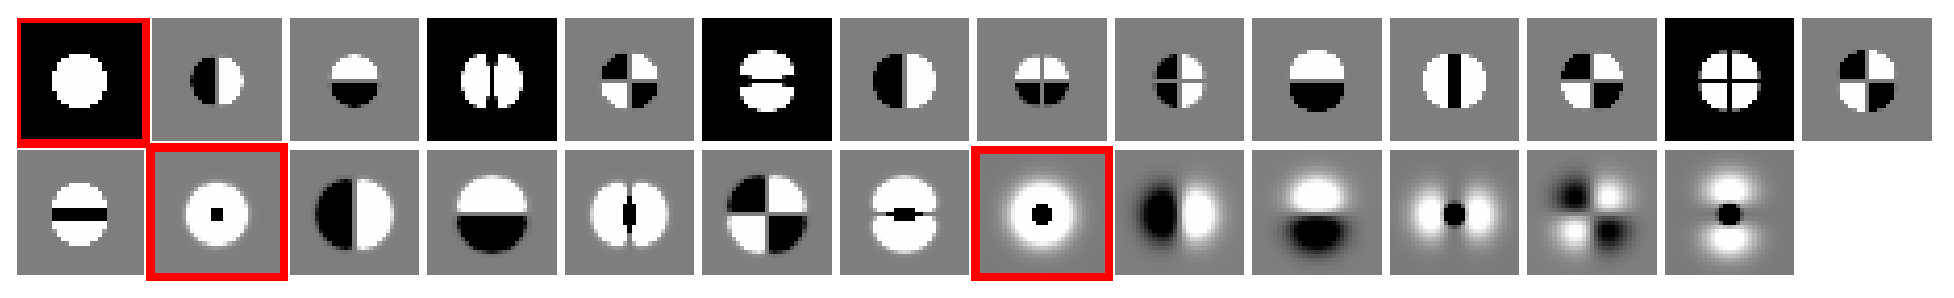
\includegraphics[width=0.8\textwidth]{figures/basis3.eps}}
\caption{Example basis set with nGauss=3 (highlighted in red),
  sigGauss=(0.5 sig, 1.0 sig, 2.0 sig), and degGauss=(4,2,2).}
\label{basis}
\end{figure}

For each source $j$ returned by DiaCatalogSourceSelector, we create a
{\tt KernelCandidate} instance, which holds substamps of $T_j(x,y)$
and $S_j(x,y)$ centered on the source.  These will be used to fit for
a local solution $K(u,v)$; the ensemble of local solutions at each
source's $x,y$ will be used to fit for the full spatial solution
$K(u,v,x,y)$.  We emphasize that the dimensions of the substamps is
important.  Note from equation~\ref{eq-soln} that the coefficients
$a_i$ are derived from a convolution of the template substamp with the
kernel basis functions $K_i$.  This convolution means that
kernelSize//2 pixels along each substamp edge are rendered unusable.
To maintain a significant number of pixels in $C_i$, we set the
KernelCandidate dimensions to be twice that of the kernel (i.e. the
number of pixels remaining in $C_i$ is equal to the number of pixels
in the kernel, which is fewer than the number of bases $i$).  For each
KernelCandidate, we solve for $K(u,v)$ and create a local difference
image $D_j(x,y)$.  We evaluate several statistics on this local
difference image, normalized by the square root of its variance, which
puts the pixels in units of sigma.  We measure the mean sigma, the RMS
of this distribution, the $\chi^2$ of these pixels normalized by the
degrees of freedom (number of pixels in $D(x,y)_j$ minus the number of
kernel bases), and the mean squared error.  These are referred to as
the LOCAL kernel metrics, and reflect how appropriate the chosen
kernel basis is.

The ensemble of {\tt KernelCandidates} is then used to constrain a
spatial model of the kernel $K(u,v,x,y)$.  This is done using the {\tt
  SpatialCellSet} formalism, whereby the {\tt KernelCandidates} are
distributed across the image in a grid of {\tt SpatialCells}.  At most
3 {\tt KernelCandidates} per {\tt SpatialCell} are input to a spatial
model of the kernel.  This formalism attempts to distribute
constraints on the spatial model evenly across the image.  For the
spatial kernel model, we assume that each of the kernel coefficients
$a_i$ may be represented by a $N^{th}$ order 2--dimensional Chebyshev.
Normally, we would perform sigma--clipping iterations on candidates
having bad residuals after spatial modeling.  However in this
production we expect that all objects should fit, so we perform no
sigma clipping.  Having generated the full spatial solution
$K(u,v,x,y) = \sum_i a_i(x,y) K_i(u,v)$, we evaluate the kernel
solution at the position of each {\tt KernelCandidate}, create a
difference image using this kernel, and recalculate the metrics
defined above.  These are referred to as the SPATIAL kernel metrics.
Importantly, we also interpolate this solution to the positions of the
control sample, which were explicitly {\it not} used in the spatial
fit, and evaluate these same metrics.  The differences between the
{\tt KernelCandidate} LOCAL and SPATIAL metrics, as well as the values
of the SPATIAL metrics for the control sample, reflect the
appropriateness of the spatial model and our ability to interpolate
and extrapolate to the full extent of the images.  We use the Mean
Square Error (MSE) of the control sample to example the tradeoff
between bias and variance in the spatial interpolation.

We next run the SourceDetectionTask on the difference image, using a
``polarity'' of {\it both} to search for both positive and negative
deviations.  We use a nominal detection threshold of 5 sigma.  In the
case of pre--filtering, we detect on the difference image directly.
In post--filtering, we correlate the difference image with its Psf (by
design, the same as the Psf of $S$) before detection is run.  All else
being equal, the images immediately preceding the detection step
($D'$) should be {\it exactly} the same.  We expect minor differences
in the variance due to the fact that the post--filtered data will have
gone through 3 convolutions (astrometric resampling; Psf--matching to
the science image; Psf filtering for detection) while the
pre--filtered data will have gone through only two (astrometric
resampling; psf--matching to the maximum likelihood image).
Differences in the shapes and sizes of the Psf--matching kernels used
in the two cases may also cause systematic differences in the images.
Detections are merged using a grow radius of 2 pixels.

Finally, we run DipoleMeasurementTask on the detections to create {\tt
  DiaSources}.  DipoleMeasurementTask is an extension of
SourceMeasurementTask that includes specific dipole measurement
algorithms.  Measurement is necessarily different in the pre--filtered
and post--filtered data.  In particular, in post--filtering, detection
happens on the filtered maximum likelihood image and source
measurement on the associated pixels in the unfiltered difference
image.  In pre--filtering, the latter does not exist, and thus
detection and measurement happen on the same image.  This restricts
the types of measurements that may be made on the sources.  In
particular, the Psf flux is merely the fitted amplitude of the peak in
the image, and the Psf centroid its center.  While these measurements
are trivial to implement, additional work needs to be done on how to
implement the remainder of the measurement suite in a manner comparable
to the measurements on post--filtered data.

All {\tt DiaSources} are associated with the {\tt calexp's} {\tt
  sources} and with the reference catalog, with a permissive matching
radius of 3''.  {\tt DiaSources} that match with {\tt sources} may be
true residuals around stars {\it or} true false detections that are
also found in {\tt calexp} SourceDetectionTask.  For this reason, we
use the associations with the reference catalog objects as the
assessment if a given {\tt DiaSource} matches with a {\tt source} or
whether it is an orphan (e.g. a statistical fluctuation in the
background).  In addition, all {\tt KernelCandidates} are persisted
with the above {\tt LOCAL} and {\tt SPATIAL} metrics.  Repositories
are accessed with a specially written RepositoryIterator that
aggregates {\tt KernelCandidates} from a given {\tt source} across
multiple output repositories.

\subsubsection{Configs {\bf ANDYB}}

We ran several pre--productions to tune: the dimensions of the kernels
and KernelCandidates; the widths of the Gaussians (sigGauss) based on
the FWHM of the input images; and the scaling of the Gaussians
($\beta$) in the basis sequence.  The main production runs included:
an outer loop over the use of pre--filtering or post--filtering for
detection; variations of the complexity of the Kernel basis, including
the number of Gaussians (nGauss = 1,3) and the degree of the modifying
Laguerre polynomials (degGauss = 1..6); and the spatial order of the
Chebyshev polynomials on $a_i(x,y)$ (spatialKernelOrder = 1..6).
Finally, we ran several post--productions focused on perturbing the
solutions that yielded the fewest numbers of DiaSources along specific
dimensions.  This included: the RMS of the WCS solution used by
RegisterTask; including a DC offset in the source positions prior to
RegisterTask, to determine the ability of the kernel basis to
accommodate astrometric misregistration; the size of the SpatialCells
used in the spatial interpolation, which effectively regulates the
numbers of constraints that go into the spatial fit; and modifying the
detection thresholds to determine how the number of false detections
scales with threshold.

\subsubsection{Measurement {\bf RUSS}}

\subsection{Simulations {\bf ANDYC}}

These algorithms were run on 3 visits, with seeings 0.6'' (visit
6866601), 0.88'' (visit 6866602), and 1.2'' (visit 6866603).  These
visits were simulated with {\bf DETAIL}.  All 9 sensors of the central
raft were simulated, for a total of 27 difference images per
configuration to use in our comparative analysis.

A template image was generated by {\bf DETAIL}.  The template has a
seeing of 0.88''.  This means that the matching of the template image
with visit 6866601 will yield a template {\it deconvolution} in the
postfilter configuration.  The matching of the template with 6866601
in the prefilter configuration, and with 6866602 in the postfilter
configuration, will yield a small convolution, since both images will
have a FWHM of 0.8--0.9''.  All other Psf--matching operations will
yield a significant convolution of the template image.

\section{KernelCandidate Statistics}

\subsection{Mean Squared Error {\bf SIMON}}

In order to investigate the bias--variance trade--off in the overall
fit, we calculate the MSE of each KernelCandidate's difference image
derived from the evaluation of the spatial model at that location.  We
define the bias as $\left| data - model \right|$, the variance as
$\left| (data - model)^2 \right|$, and the MSE as {\tt bias$^2$ +
  variance}.  In this context, the bias is the mean of the difference
image, and the variance is the mean square of the difference image.
In both cases, we normalize by the square root of the variance so that
pixels are in units of sigma.

\subsection{Reduced $\chi^2$ {\bf SIMON}}

\subsection{Control Sample {\bf SIMON}}

\section{False Detection Rate}

\subsection{Theoretical {\bf ANDYC}}

\subsection{Empirical {\bf ANDYB}}

After running an ensemble of 144 pipeline configurations, we
aggregated the numbers of false detections.  We report the results for
the each of the 3 visits, and for pre-- and postfiltering for
detection.  We cut on {\tt flags.pixel.edge} to remove spurious
detections on the immediate border of the image; other than that we do
no other cuts other than requiring that the {\tt centroid.sdss} is
finite.  We count the DiaSources that match with the reference catalog
(3'' matching radius) via the {\tt refMatchId} value.  We find no
significant correlation of false detections with sensor within the
raft; therefore we report the aggregate results for all 9 sensors in
the analysis that follows.

A set of ``heat maps'' are presented in Figure~\ref{fp_heatmap}, that
demonstrate the total number of detections across all 9 sensors as a
function of the config parameters spatialKernelOrder and degGauss, for
nGauss = 3.  Qualitatively, these heat maps indicate that a Chebyshev
spatial order greater than 3 is required for all data.  In addition,
with the exception of the deconvolution case (visit 6866601 and
prefilter=False), the Gaussians need to be modified by Laguerre
polynomials of order 4 or higher.  The minimum of these detection maps
are found using the configs of highest complexity, with a very flat
slope in the number of false detections beyond spatialKernelOrder$>$3
and degGauss$>$3.  There is not much evidence for an upturn in the
numbers of false detections, meaning we have likely not reached the
case of overfitting using these configs.

The numbers of false detections in each best case are given in
Table~\ref{tab-bestfp10a}.  We undertook a manual inspection of all
difference images to associate the DiaSources with Sources in the
images, and also a 3'' association with the input source catalog.
These associations are listed in the N$_{Match}$ column of
Table~\ref{tab-bestfp10}, with the unmatched false positives in the
N$_{Orphan}$ column.  The former are likely to come from systematics
in the subtractions of stars, while the latter would be due to
fluctuations in the background.  We note 2 effects that will impact
N$_{Match}$.  The first is that, with a 3'' matching radius, 4\% of
random fluctuations will by--chance associate with a Source.  Assuming
that N$_{Orphan}$ represents 96\% of the background fluctuation
population, we estimate the number of fluctuations from that same
population that would have associated with Sources as N$_{Random}$.
Finally, we count all matches that occur within 100 pixels of the
image boundary, where we might expect the spatial extrapolation to
yield systematic residuals, as N$_{D<100}$.  To the extent that
(N$_{Random}$ + N$_{D<100}$) < N$_{Match}$, we have a small residual
set of systematic false detections in our imaging ensemble.  Aside
from the deconvolution run, this is at the level of 10 total false
detections over 9 sensors in 5 production runs, or 1 every 4--5
images.

We also list the ratio of negatively detected to
positively detected DiaSources.  That this ratio is significantly
greater than 1.0 in most cases suggests that there is an
over-subtraction of the background in the process, which biases this
ratio (see Section~\ref{sec-bg}).  The optimal configurations yielding
these false detection rates are given in Table~\ref{tab-bestconfig10}.

We have examined the distribution of these false detections across the
image, and find no significant overdensities near the borders of the
images, which would be expected in cases of under or over--fitting of
the various spatial models (astrometry, backgrounds, Psf--matching
kernels).  Figure~\ref{edgedist} provides the distribution of
distances from the edge of the sensor for all false detections in {\it
  blue}, with a random sample of points in the image given in {\it
  green}.  Uncertainties are plotted using the square root of the
number of points in each bin, and the histograms are normalized to
provide a probability density.  The takeaway is that we find no
significant correlation of false detections with the boundaries of the
fitting functions.

\section{False Detection Dependencies}

After finding the configurations that yielded the minimal numbers of
false detections, we then perturbed the solutions to examine how the
numbers of false detections scaled with different effects.  This
included, in order of importance for this production: the difference
image detection threshold; the number of KernelCandidates going into
the spatial model; and astrometric registration errors.  We also
undertake a theoretical analysis of the number of false detections
expected in a 4k x 4k image as a function of detection threshold, and
examine the requirements this sets on our ability to model the
variance and backgrounds in the images.  We compare the empirical
variation of false detections with detection threshold, and show that
our data are consistent with this.

\subsection{Detection Threshold {\bf SIMON}}

To estimate the numbers of false detections we would expect in a
$4000\times4072$ pixel science image with a given FWHM in pixels, we
do the following.  The theoretical expectations for the number of
false detections due to random Gaussian fluctuations is outlined in
\cite{Kaiser-PointSources}.

\subsection{Number of KernelCandidates {\bf ANDYB}}

\subsection{Registration Errors {\bf ANDYB}}

We implemented two simple perturbations of the inputs to the
image--to--image RegisterTask: we first added a random offset to each
object's (x,y)-coordinates, with an amplitude that was specified in
the Config and multiplied by a random number pulled from a normal
distribution; and we added a DC offset to the coordinates at an
amplitude specified in the Config.  These offsets, added to the Source
coordinates, will affect misalignments of the objects in the
registered images, as the registration is done assuming the specified
positions are correct.  In this way we are able to investigate how
random uncertainties and bulk astrometric offsets impact the false
positive rate.  We explicitly do {\it not} investigate spatial
variation in these offsets, using for example a pincushion distortion.
We anticipate that this latter effect will be most important for
spatial interpolation and extrapolation of the matching kernel,
yielding a dipole residual field associated with the distortion.
However, the ability of the software to model out these spatial
distortions will certainly fail if the local kernel solutions (from
which the spatial model is derived) are unable to compensate for
misalignments.

%\begin{figure}
%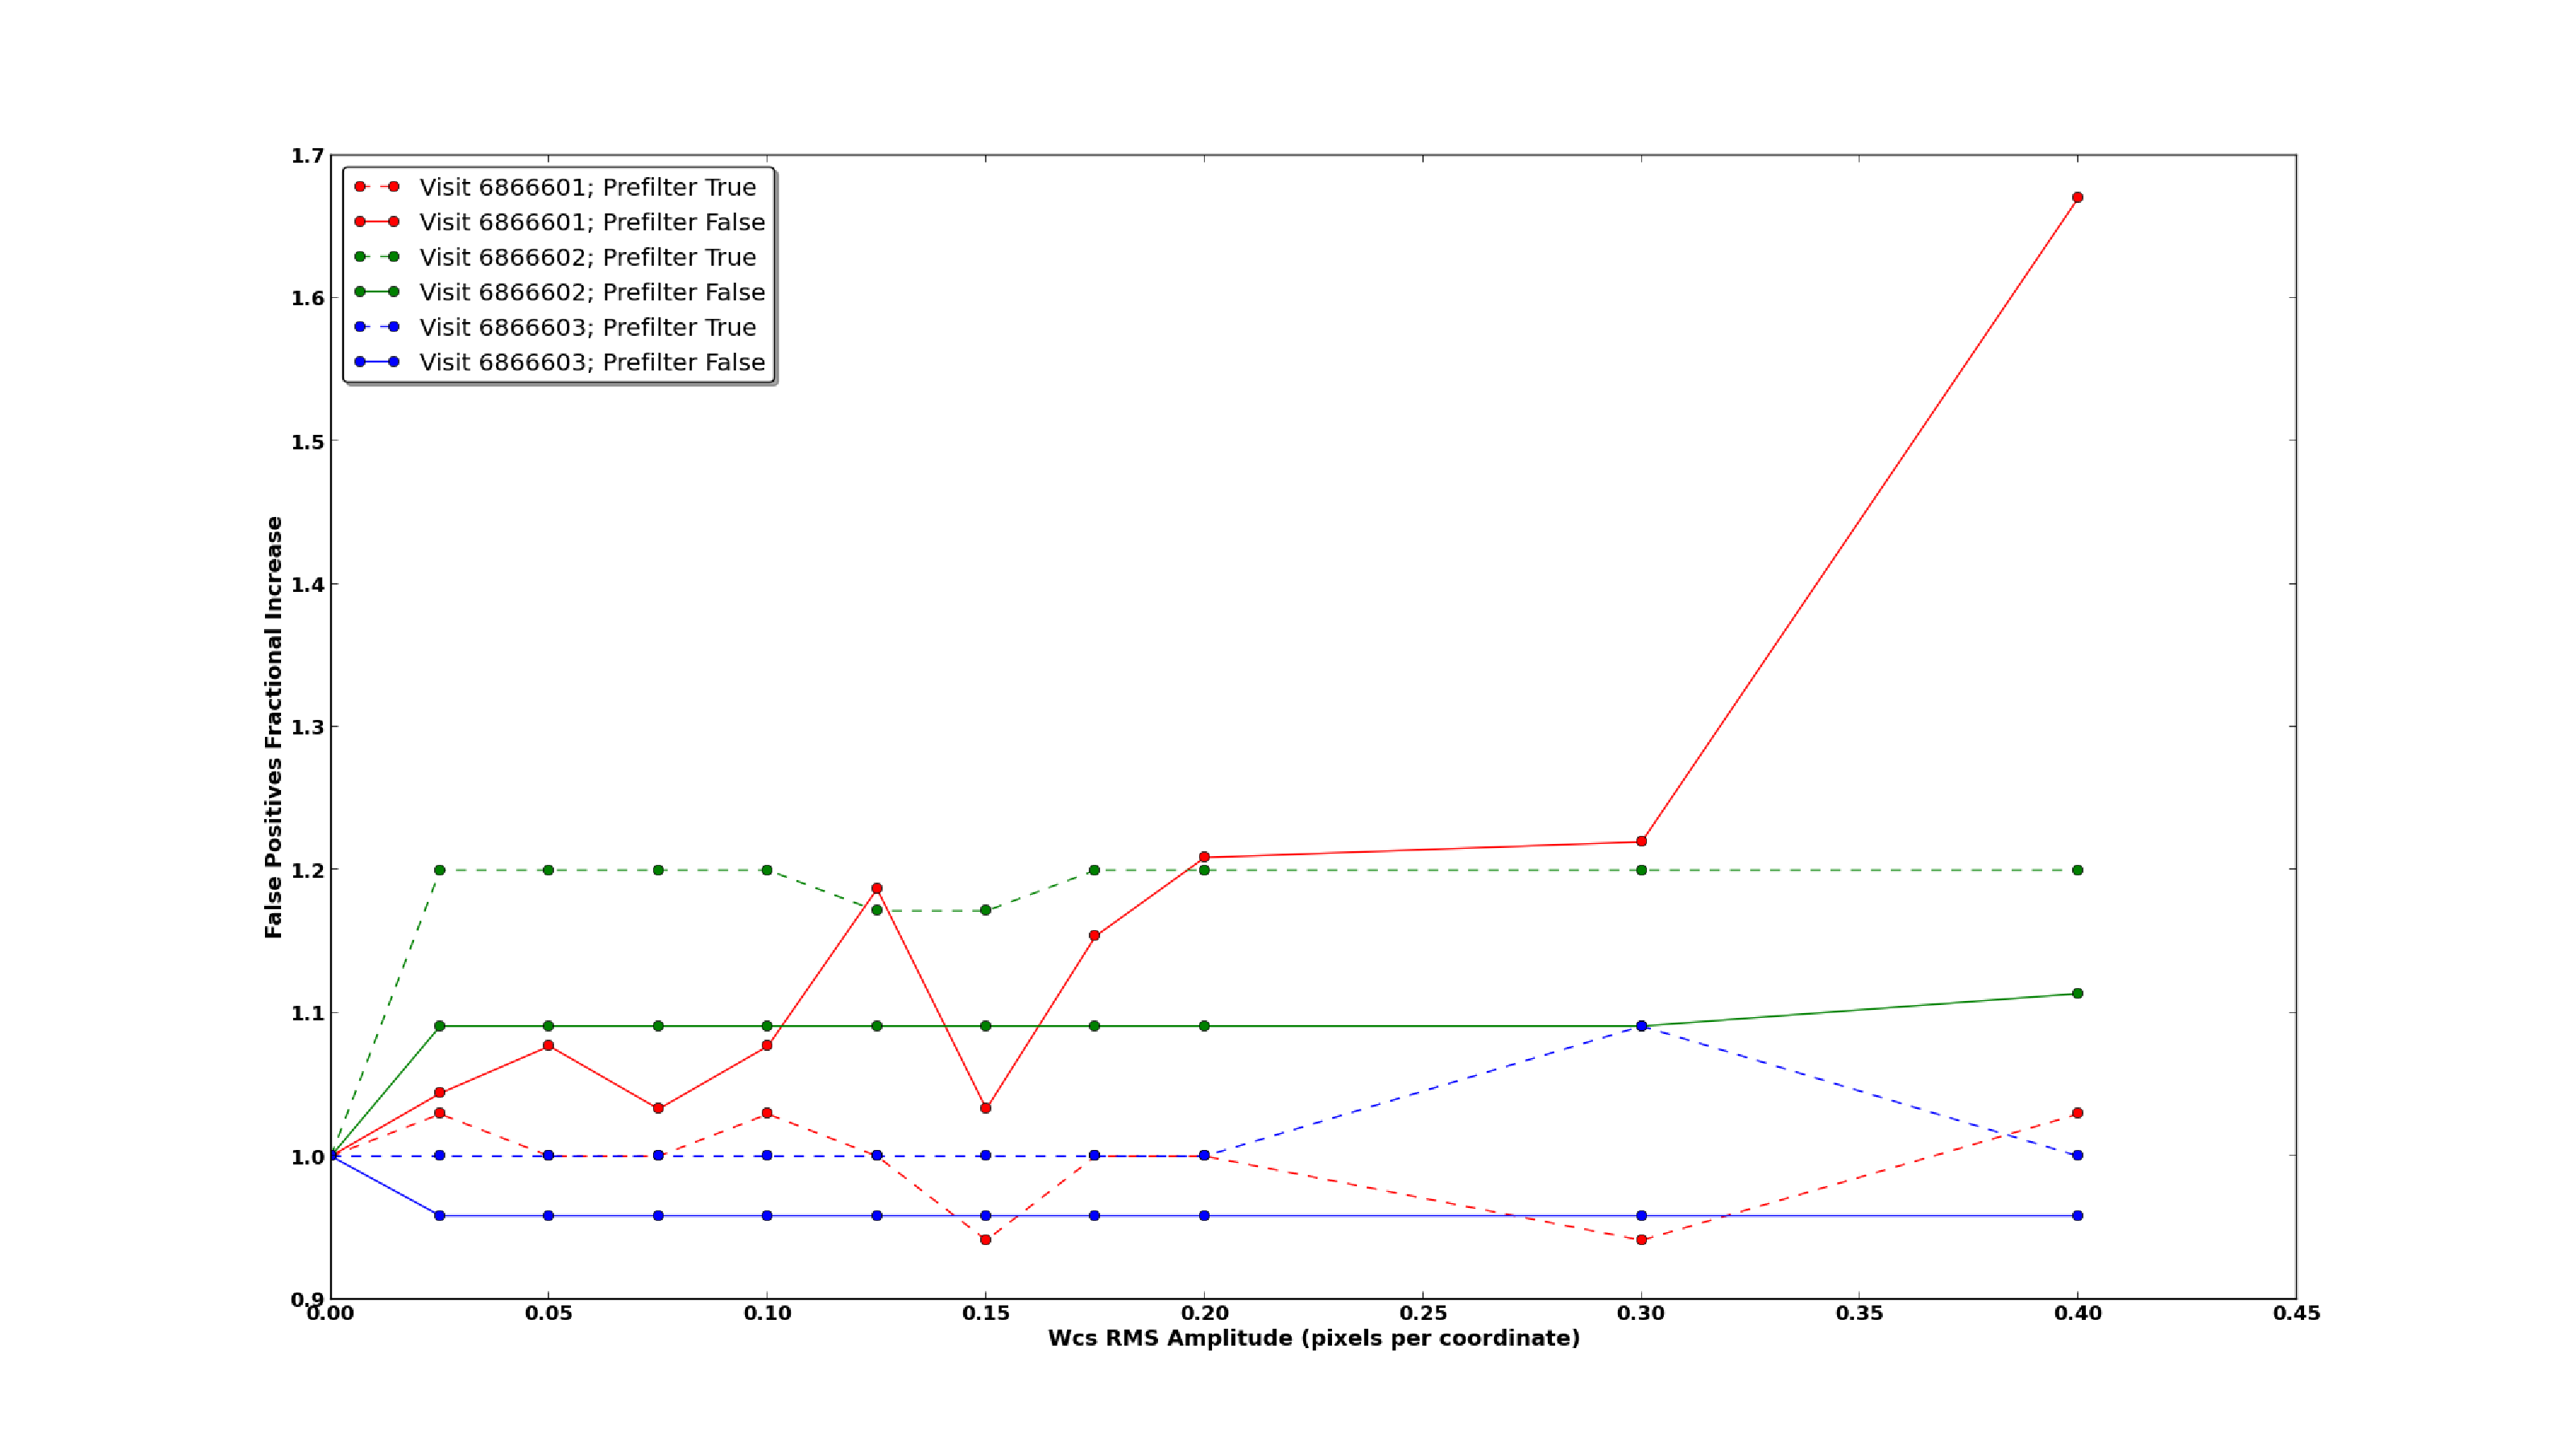
\includegraphics[width=0.5\textwidth]{figures/wcs_rms.eps} 
%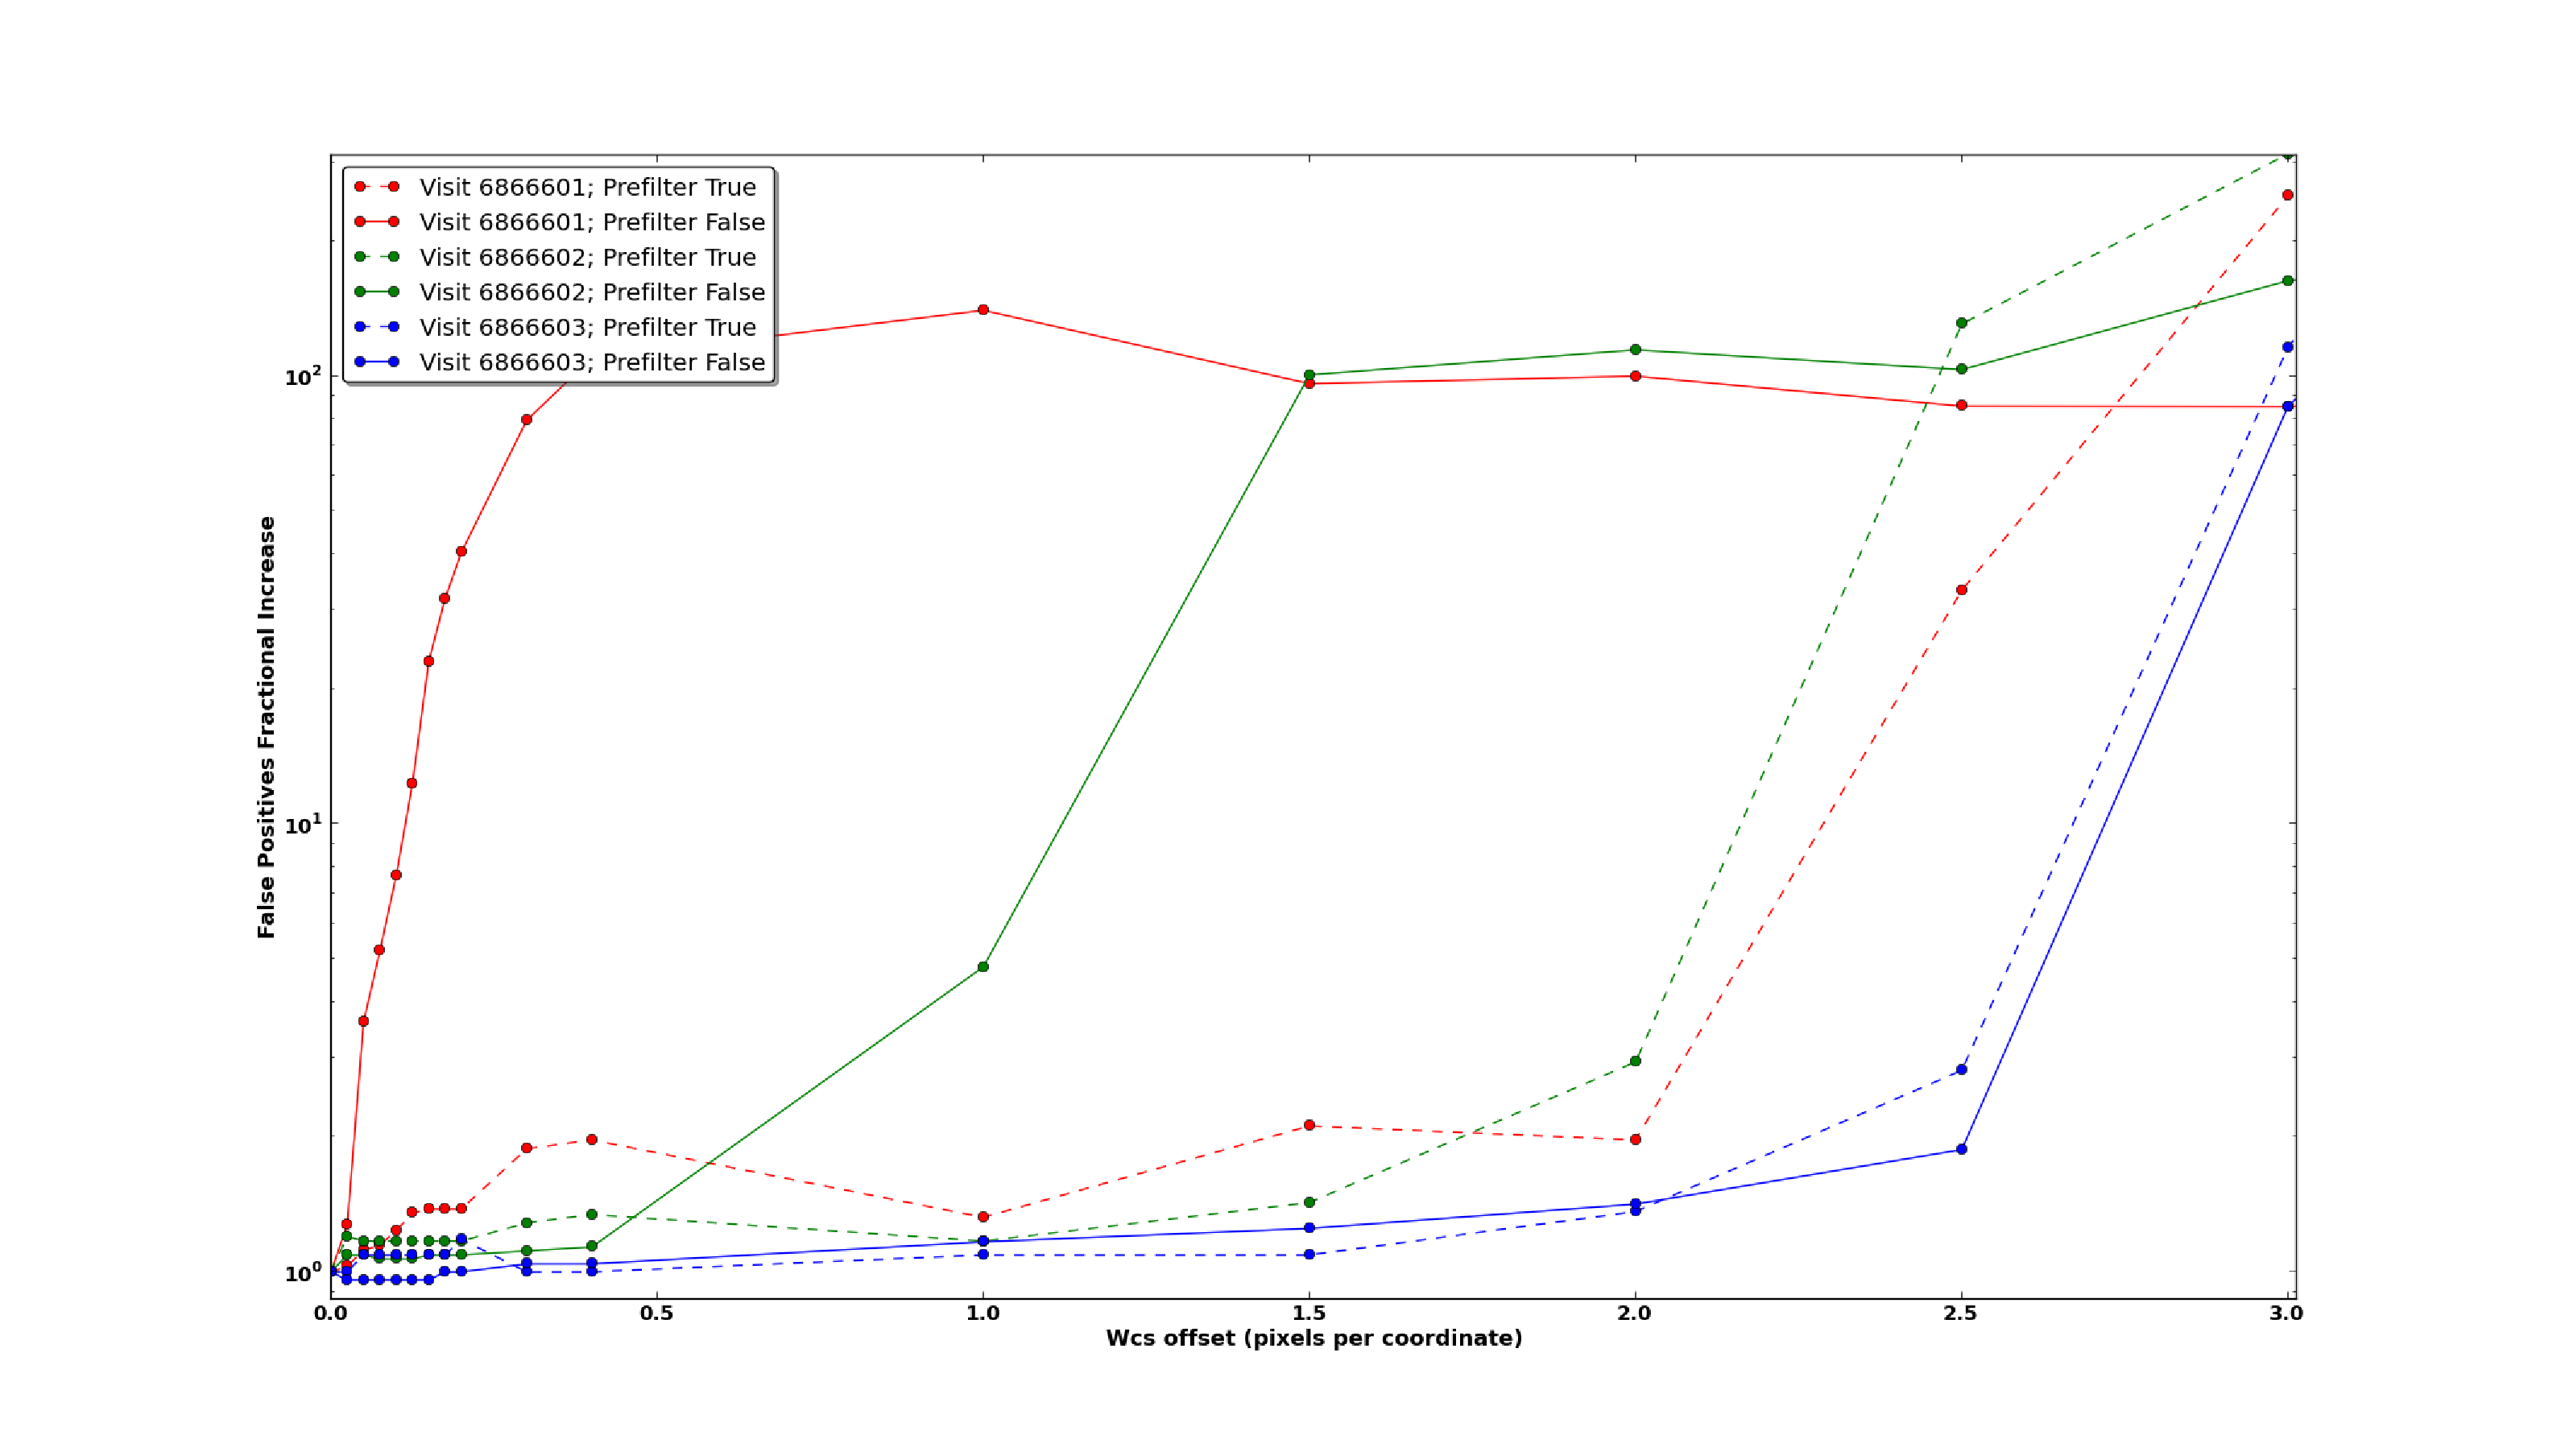
\includegraphics[width=0.5\textwidth]{figures/wcs_offset.eps} \\
%\caption{WCS}
%\label{wcs_offsets}
%\end{figure}

\subsubsection{Coordinate RMS {\bf ANDYB}}

We perturbed the coordinates of each template Source that was input to
RegisterTask with amplitudes of (0.025, 0.05, 0.075, 0.1, 0.125, 0.15,
0.175, 0.2, 0.3, 0.4) pixels, and to randomize the effects we
multiplied each offset by a number pulled from a normal (0,1)
distribution.  The output RMS reported by RegisterTask was noted to
track these offsets.


\subsubsection{Coordinate Offsets {\bf ANDYB}}

We offset the coordinates of each template Source that was input to
RegisterTask with amplitudes of (0.025, 0.05, 0.075, 0.1, 0.125, 0.15,
0.175, 0.2, 0.3, 0.4, 1.0, 1.5, 2.0, 2.5, 3.0, 3.5, 4.0) pixels.
Post--registration, this will offset the positions of sources in the
two images by the desired amount.

\subsection{Background Subtraction {\bf SIMON}}

\subsection{Variance Misestimation {\bf ANDYB/SIMON}}

The variance in the prefiltered and postfiltered images is likely to
be different due to the different types of operations that have
happened on the images.  We quantify this by taking the postfiltered
images, immediately before the detection step (i.e. $D'$), and compare
the variance plane to that coming from the prefiltered image
(Table~\ref{tab-variance2}).  For v6866601, which is a deconvolution
in the postfiltered production, we find that the variance is 70\%
higher when postfiltering.  This is consistent with the expectation
that deconvolution increases the noise properties of the image.  For
v6866602 and v6866603, we find that the variance is 3--4\% and 2--3\%
higher in the {\it prefiltered} data, respectively.  The primary
culprit for this is that the prefiltered data will have gone through 1
less convolution, meaning less of the variance will have been lost to
covariance.

To quantify the significance of these offsets, we compared the
empirical variance in the image planes with the variance tracked by
the variance planes to ascertain how much we are misestimating the
true variance.  We calculated the ratio of the interquartile range of
unmasked pixels in the image plane, multiplied by 0.741 and then
squared, with the median of unmasked pixels from the variance plane.
The results are summarized in Table~\ref{tab-variance1}.  We find that
we are marginally, but consistently, underestimating the variance in
our images by $\sim 1\%$.  This affect is smaller than the amplitudes
reported above, indicating that there are true differences in the
variances of prefiltered and postfiltered detection images.

\section{Conclusions}

We can reach near the theoretical limit for false detection rate in
these ideal data, something which has not been demonstrated for image
subtraction algorithms in the past.

Pre--filtering is clearly preferred when the traditional process would
lead to deconvolution, or sharpening, of the data.  When the standard
processing results in a convolution, or smoothing of the data,
pre--filtering provides fewer false detections.  As a trade--off, the
measurement of these false detections is not yet well defined.

\begin{itemize}

\item We find that the overall number of false detections is not
  strongly sensitive to bulk background misestimation
  (Figure~\ref{XXX});

\item However, the ratio of positive to negative false detections is
  strongly dependent on background fitting, with {\bf XXX}
  (Figure~\ref{XXX}).

\item Our empirical negative to positive false detection ratio is {\bf
  X.X}, indicating a bias in the background levels of {\bf X\%}.

\item At the 5--sigma detection threshold, for the range of seeings
  considered in this production, the theoretical numbers of false
  detections per 4k x 4k sensor numbers 10+.  This function is steep;
  by increasing the detection threshold to 5.X sigma this number may
  be lowered to less than 1 per sensor.

\item Due to the steepness of this function, the number of false
  detections is strongly dependent on the variance being correct, at
  the 5--sigma detection threshold.  When detecting at 5--sigma,
  having the variance underestimated by 1\% leads to an increase
  in false positives of {\bf XXX} (Figure~\ref{}).

\item An empirical computation of the variance from the image plane,
  compared to the median propagated variance in the variance plane,
  indicates that we consistently underestimate the variance by $1-2\%$
  (Table~\ref{tab-variance1}).  A proper tracking of covariance during
  the multiple image convolutions that occur may alleviate this
  problem.

\item When convolving to Psf--match, variance planes of postfiltered
  detection images have {\it lower} variance than their prefiltered
  counterparts by $2-3\%$ (Table~\ref{tab-variance2}).  These images
  have gone through one additional convolution compared to the
  prefiltered data.

\item When deconvolving, the postfiltered variance is 70\% {\it
  higher} at the time of detection compared to the prefiltered data
  (Table~\ref{tab-variance2}).  This is consistent with the
  understanding that deconvolution increases high frequency noise in
  the images, and provides a {\it lower} detection efficiency in
  deconvolved data.  Prefiltering is clearly preferred in the case of
  deconvolution.

\item The false detection rate is seen to scale with detection
  threshold in a manner consistent with theory (Figure~\ref{}).

\item Several statistics that we are able to calculate at the time of
  image subtraction are shown to correlate strongly with the numbers
  of false detections, providing real--time quality estimates
  (Figures~\ref{}).

\item The numbers of false detections that associate with Sources is
  shown to correlate with the amount of smoothing that occurs in the
  Psf matching, in the sense that more smoothing leads to fewer false
  detections (Figure~\ref{}).  In this sense, there is a strong
  preference for running in prefiltered mode.

\item Measurements on prefiltered difference images contain less
  information than in postfiltered difference images, because the
  paradigm of detection on filtered data but measurement on the
  unfiltered data is broken.  Thus while we detect on average fewer
  false positives in prefiltered data, we are (so far) able to
  characterize them less well.  This trade--off is clearly something
  to explore in future work.

\end{itemize}

\section{Future Work}

We intend to research additional aspects of the problem going forward,
including:
\begin{itemize}
\item How the false detection rate varies with more realistic SEDs;
\item How the false detection rate varies with airmass;
\item How the system behaves with a realistic mix of stars and galaxies;
\item How the false detection rate looks in crowded fields;
\item How to perform measurement on pre--filtered difference images;
\end{itemize}

\clearpage
\bibliographystyle{apj}
\bibliography{refs}

\clearpage
%\begin{table}
%\centering
%\begin{tabular}{clcc}
%\hline
%\multicolumn{4}{|c|}{Best Results: Production 8} \\
%\hline
%Visit    & Prefilter & False Detection Matches & False Detection Orphans \\
%\hline
%v6866601 & True      & 5                      & 29  \\
%         & False     & 10                     & 81  \\
%v6866602 & True      & 5                      & 30  \\
%         & False     & 9                      & 35  \\
%v6866603 & True      & 2                      & 9   \\
%         & False     & 1                      & 23  \\
%\end{tabular}
%\caption{Total number of {\tt DiaSources} detected at 5--sigma from
%  all 9 sensors in raft 2,2, for the configurations that yielded the
%  lowest number of false detections.  Matches are determined using a
%  3'' match radius with the input reference catalog.  Objects with the
%  {\tt EDGE} flag are ignored. \label{tab-bestfp8}}
%\end{table}

\begin{table}
\centering
\begin{tabular}{clcccccc}
\hline
\multicolumn{8}{|c|}{Best Results: Production 10} \\
\hline
Visit    & Prefilter & Total False Detections &  N$_{Orphan}$ & N$_{Match}$ & N$_{Random}$ & N$_{D<100}$ & Nneg / Npos \\
\hline
v6866601 & True      & 70      &60         & 10 & 3     & 4   & 1.8 \\ 
         & False     & 143     &51         & 92 & 2     & 11  & 0.4 \\
v6866602 & True      & 42      &36         & 6  & 2     & 1   & 2.6 \\
         & False     & 53      &45         & 8  & 2     & 1   & 0.5 \\
v6866603 & True      & 23      &23         & 0  & 1     & 0   & 2.8 \\
         & False     & 36      &35         & 1  & 1     & 0   & 3.4 \\
\end{tabular}
\caption{Total number of {\tt DiaSources} detected at 5--sigma from
  all 9 sensors in raft 2,2, for the configurations that yielded the
  lowest number of false detections.  Matches are determined using a
  3'' match radius with the input reference catalog.  Objects with the
  {\tt EDGE} flag are ignored.  We list the number of background
  fluctuations that are expected to randomly associate with a Source
  N$_{Random}$, given the density of objects in the images and a 3''
  match radius, assuming that N$_{Orphan}$ represents 96\% of the
  total population of detections arriving from Gaussian fluctuations.
  We also list the number of false detections that are found within
  the outer 100 pixels of the image N$_{D<100}$.  The final column
  lists ratios of the number of negatively detected false detections
  to those with positive flux, a 5--sigma. \label{tab-bestfp10a}}
\end{table}

\begin{table}
\centering
\begin{tabular}{clccc}
\hline
\multicolumn{5}{|c|}{Best Results: Production 10} \\
\hline
Visit    & Prefilter & False Detections: Matches & False Detections: Orphans & Nneg / Npos \\
\hline
v6866601 & True      & 11                        & 59  & 1.8 \\ 
         & False     & 99                        & 44  & 2.9 \\
v6866602 & True      & 7                         & 35  & 2.2 \\
         & False     & 8                         & 45  & 0.7 \\
v6866603 & True      & 1                         & 22  & 2.8 \\
         & False     & 1                         & 35  & 3.0 \\
%v6866601 & True      & 11                        & 70  & 1.8 \\ SUBTRACT ME!
%         & False     & 99                        & 143 & 2.9 \\
%v6866602 & True      & 7                         & 42  & 2.2 \\
%         & False     & 8                         & 53  & 0.7 \\
%v6866603 & True      & 1                         & 23  & 2.8 \\
%         & False     & 1                         & 36  & 3.0 \\
\end{tabular}
\caption{Total number of {\tt DiaSources} detected at 5--sigma from
  all 9 sensors in raft 2,2, for the configurations that yielded the
  lowest number of false detections.  Matches are determined using a
  3'' match radius with the input reference catalog.  Objects with the
  {\tt EDGE} flag are ignored.  The final column lists ratios of the
  number of negatively detected false detections to those with
  positive flux. \label{tab-bestfp10b}}
\end{table}

%\begin{table}
%\centering
%\begin{tabular}{clccc}
%\hline
%\multicolumn{5}{|c|}{Best Configs: Production 8} \\
%\hline
%Visit    & Prefilter & nGauss & degGauss & spatialOrder \\
%\hline
%v6866601 & True      & 3      & 6        & 5 \\
%         & False     & 3      & 2        & 4 \\
%v6866602 & True      & 3      & 6        & 5 \\
%         & False     & 3      & 5        & 5 \\
%v6866603 & True      & 3      & 6        & 4 \\
%         & False     & 3      & 6        & 4 \\
%\end{tabular}
%\caption{Configurations that led to the best results listed in
%  Table~\ref{tab-bestfp8}.  All post-production runs include
%  perturbations about these configurations. \label{tab-bestconfig8}}
%\end{table}

\begin{table}
\centering
\begin{tabular}{clccc}
\hline
\multicolumn{5}{|c|}{Best Configs: Production 10} \\
\hline
Visit    & Prefilter & nGauss & degGauss & spatialOrder \\
\hline
v6866601 & True      & 3      & 6        & 6 \\
         & False     & 3      & 1        & 5 \\
v6866602 & True      & 3      & 6        & 6 \\
         & False     & 3      & 6        & 5 \\
v6866603 & True      & 3      & 5        & 5 \\
         & False     & 3      & 4        & 6 \\
\end{tabular}
\caption{Configurations that led to the best results listed in
  Table~\ref{tab-bestfp10}.  All post-production runs include
  perturbations about these configurations. \label{tab-bestconfig10}}
\end{table}


\begin{table}
\centering
\begin{tabular}{clcc}
\hline
\multicolumn{4}{|c|}{Variance Ratios} \\
\hline
Visit    & Prefilter & Mean Ratio & RMS Ratio \\
\hline
v6866601 & True      & 1.019      & 0.005    \\
         & False     & 1.011      & 0.002    \\
v6866602 & True      & 1.007      & 0.001    \\
         & False     & 1.010      & 0.002    \\
v6866603 & True      & 1.008      & 0.001    \\
         & False     & 1.015      & 0.003    \\
\end{tabular}
\caption{Ratio of the empirical variance in the difference images,
  calculated via (0.741 times the interquartile range)$^2$, to the
  median of the variance plane.  In all cases the variance plane
  represents an {\it underestimate} of the true variance in the
  images.  We report the mean and RMS across all sensors.  }
\label{tab-variance1}
\end{table}

\begin{table}
\centering
\begin{tabular}{ccc}
\hline
\multicolumn{3}{|c|}{Variance Ratios} \\
\hline
Visit    & Mean Postfilter/Prefilter & RMS Postfilter/Prefilter \\
\hline
v6866601 & 1.72      & 0.04     \\
v6866602 & 0.967     & 0.001    \\
v6866603 & 0.975     & 0.002    \\
\end{tabular}
\caption{Ratios of the variance planes immediately before detection
  $D'$.  Ratios are in the sense of the variance of the postfiltered
  image divided by the variance of the prefiltered image.  We report
  the mean and RMS across all sensors.}
\label{tab-variance2}
\end{table}


\clearpage

\begin{figure}
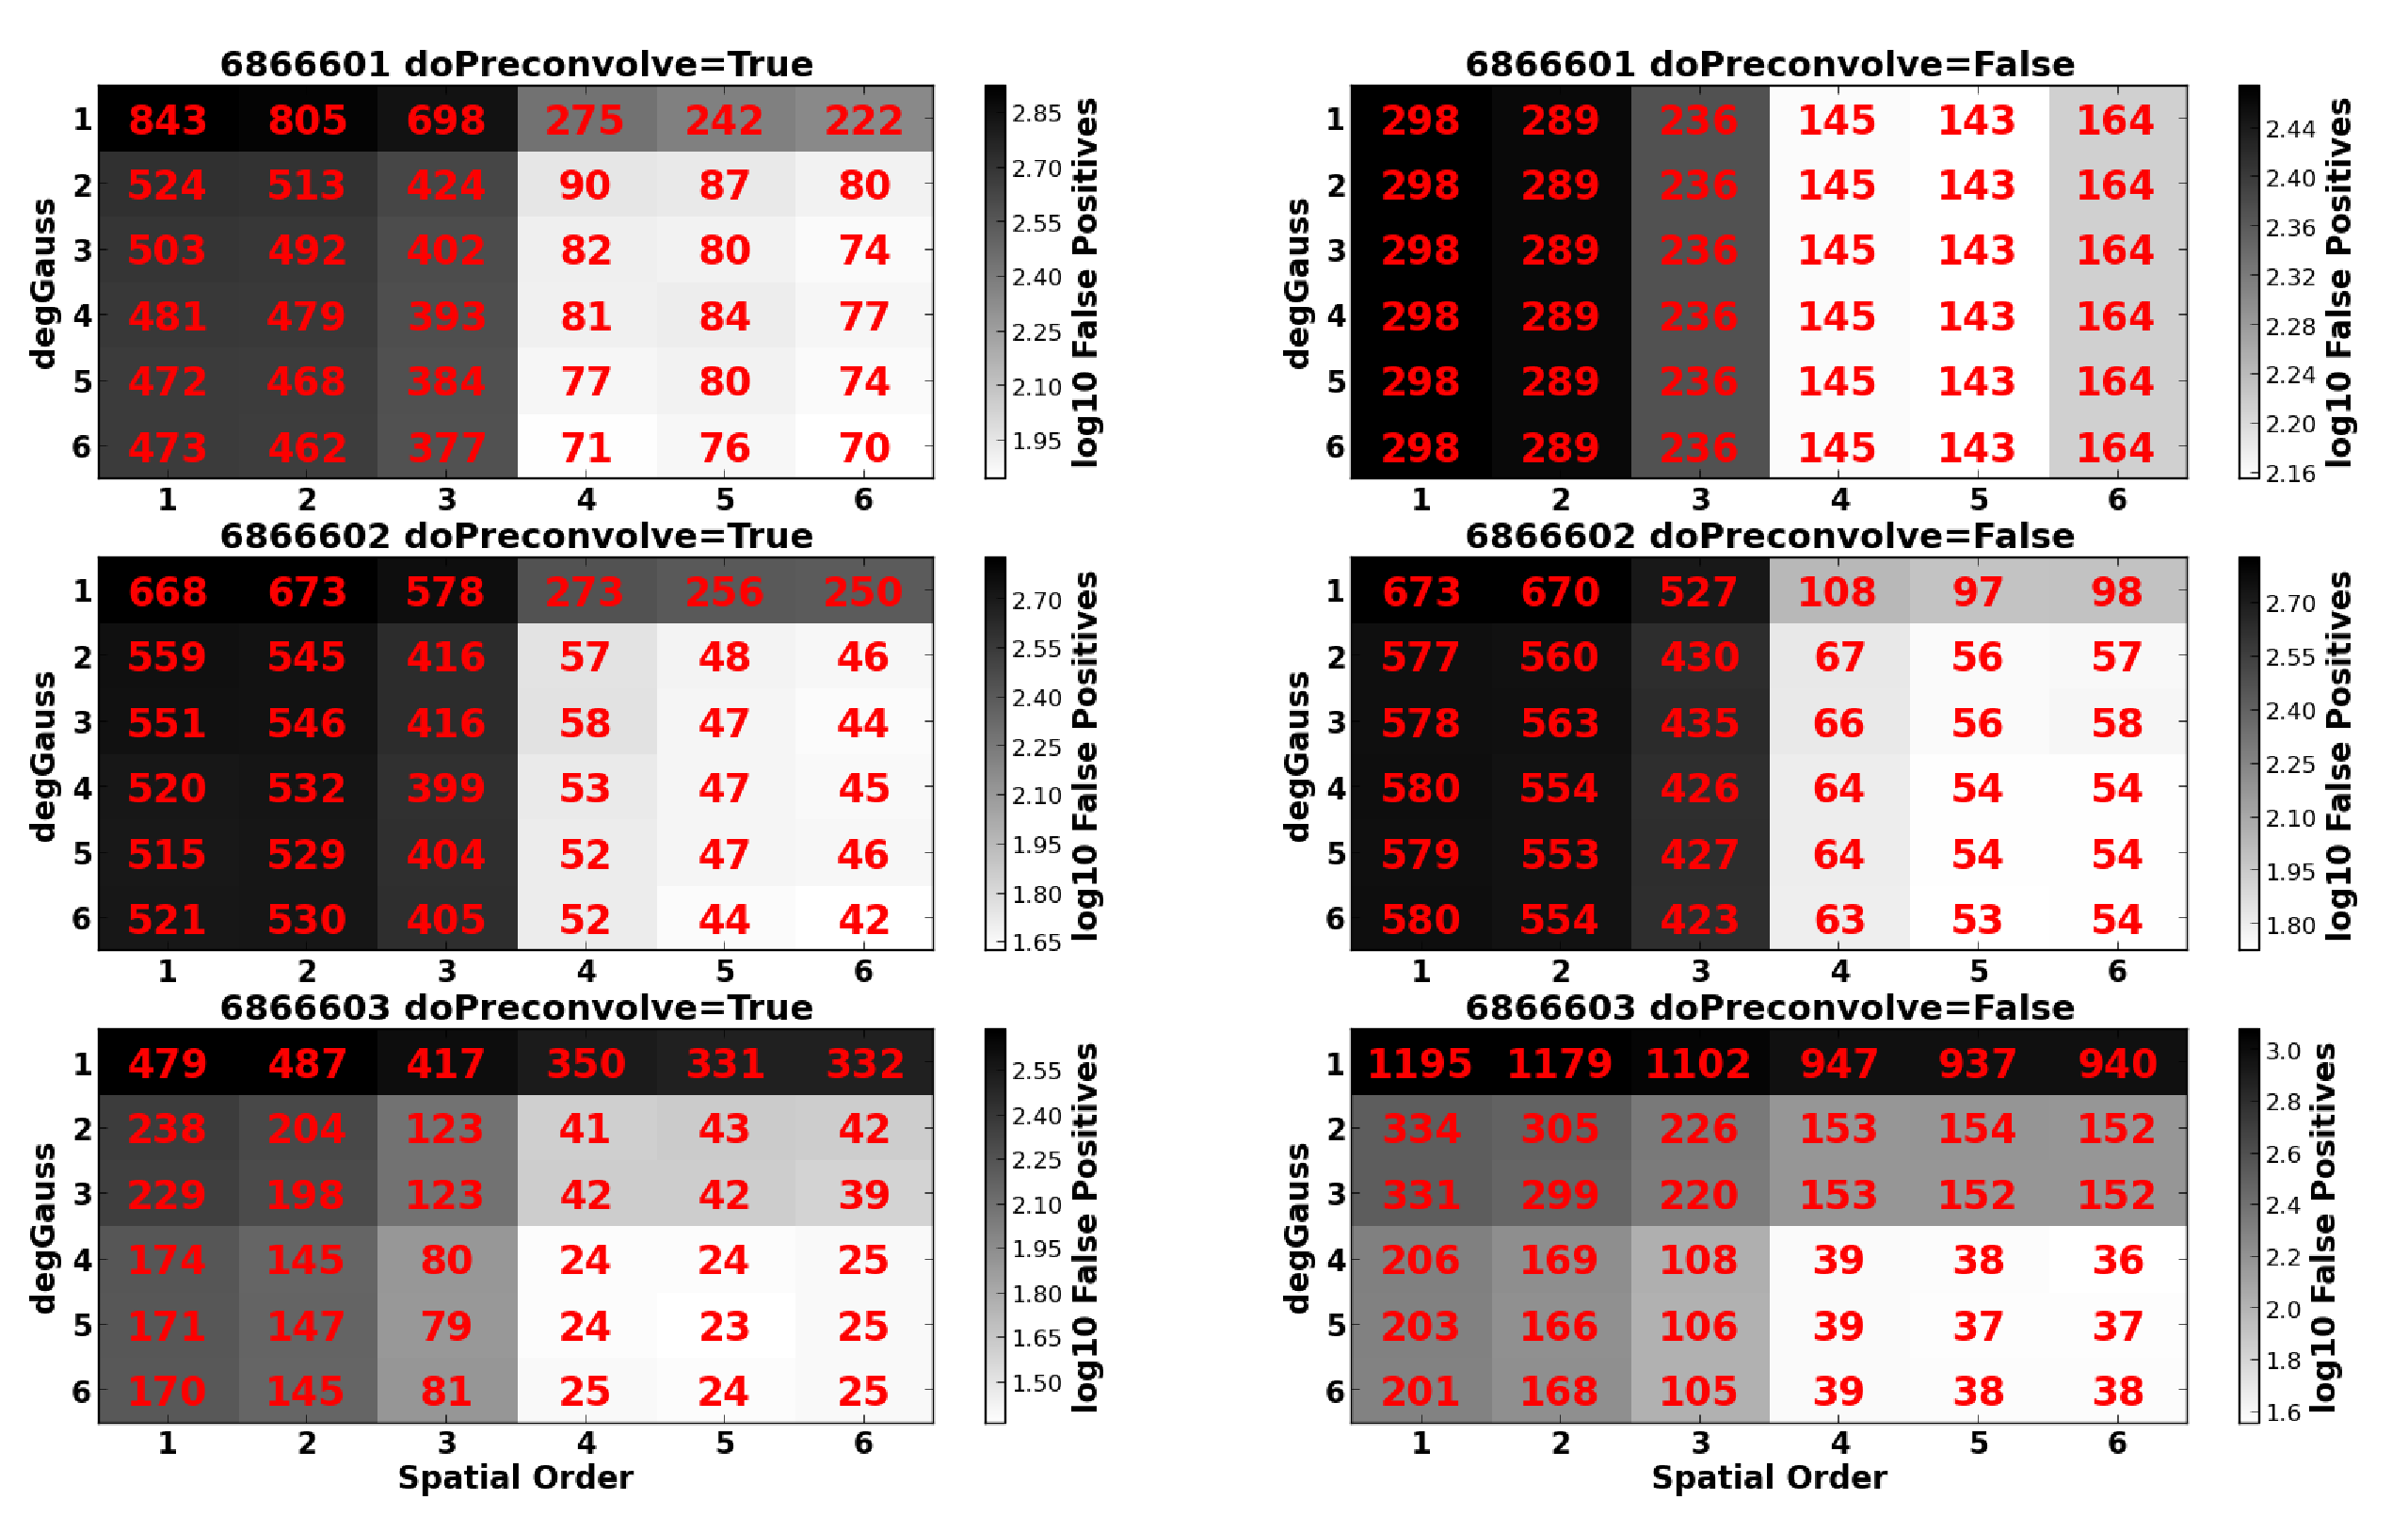
\includegraphics[width=1.0\textwidth]{figures/heatmap10.eps} \\
\caption{``Heat--map'' detailing the total numbers of 5--sigma false
  positives as a function of two main degrees of freedom: the maximum
  order of basis Laguerre polynomials along the y--axis, and the
  spatial order of the Chebyshev expansion of the spatial model along
  the x--axis.  The {\it left} column shows these results for
  prefiltering, while the {\it right} column shows this for the
  post--filtered analysis.  The best results listed in
  Table~\ref{tab-bestfp}, with the associated configurations from
  Table~\ref{tab-bestconfig}, correspond to the minimum in each of the
  subpanels.  }
\label{fp_heatmap}
\end{figure}

\begin{figure}
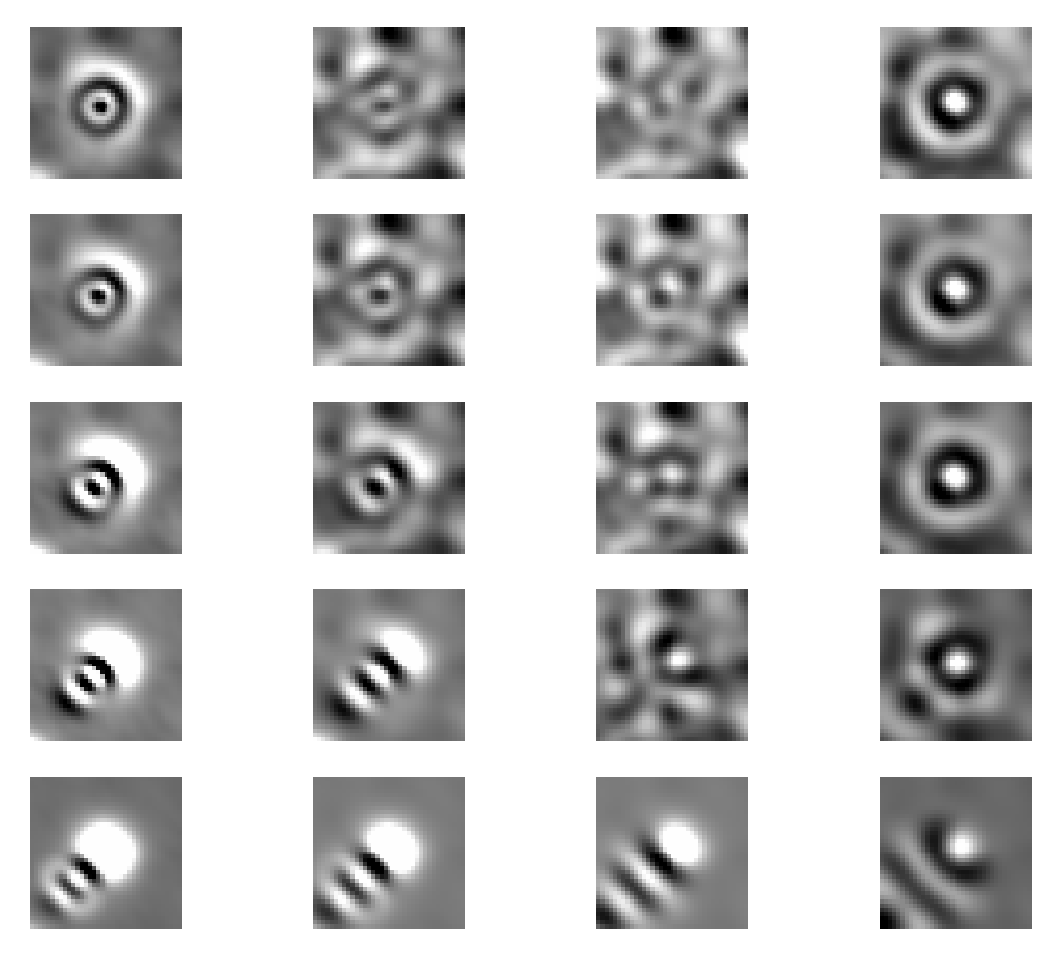
\includegraphics[width=0.8\textwidth]{figures/shift.eps} \\
\caption{Figure illustrating the ability of the kernel basis to
  compensate, locally, for the effects of misregistration.  Each
  element of the grid shows a single KernelCandidate local difference
  image (visit=6866603, doPreFilter=True).  Columns indicate the
  Gaussian sigma of the basis, which is designed to have one Gaussian
  with the prescribed width, modified to fourth order.  Rows indicate
  the amplitude of the astrometric offset that was introduced into
  the Source positions before image-to-image registration.  
  In the {\it top} row, we see that even with a small astrometric
  offset, the sigma=2 basis is unable to produce a quality
  subtraction, because the width is inappropriate for matching the two
  input Psfs (the theoretical Gaussian sigma here is 3.4 pixels).  At
  sigma=4 the basis is able to produce a quality subtraction, and by
  sigma=5 the basis is too large to match the Psfs.  In {\it row 4},
  we show that even for an astrometric offset of 4 pixels (0.8''), the
  sigma=4 basis can produce a reasonable difference image without
  structured residuals.  However, by {\it row 5}, with an offset of 6
  pixels, none of the Gaussians provide a successful local difference
  image. 
  The ability of the basis to compensate for bulk astrometric offsets
  is a function of the kernel width, and the kernel width is itself a
  function of the two input Psf FWHMs.  Thus there is a complicated
  dependence of the ability of the kernel to shift the centroids of
  stars.  Roughly, the basis may compensate for local astrometric residuals
  at a scale up to $\sqrt{\sigma_S^2 - \sigma_T^2}$.
}
\label{kernel_offsets}
\end{figure}

\begin{figure}
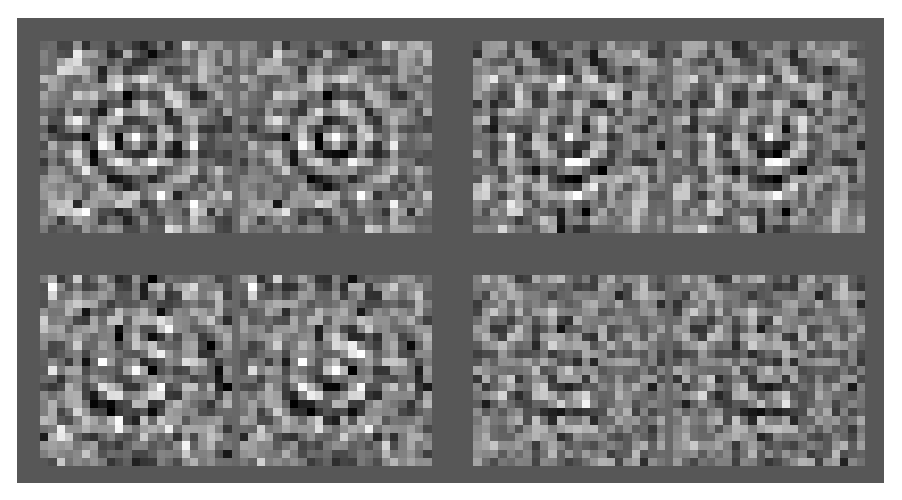
\includegraphics[width=0.5\textwidth, height=0.25\textwidth]{figures/deconv2.eps} 
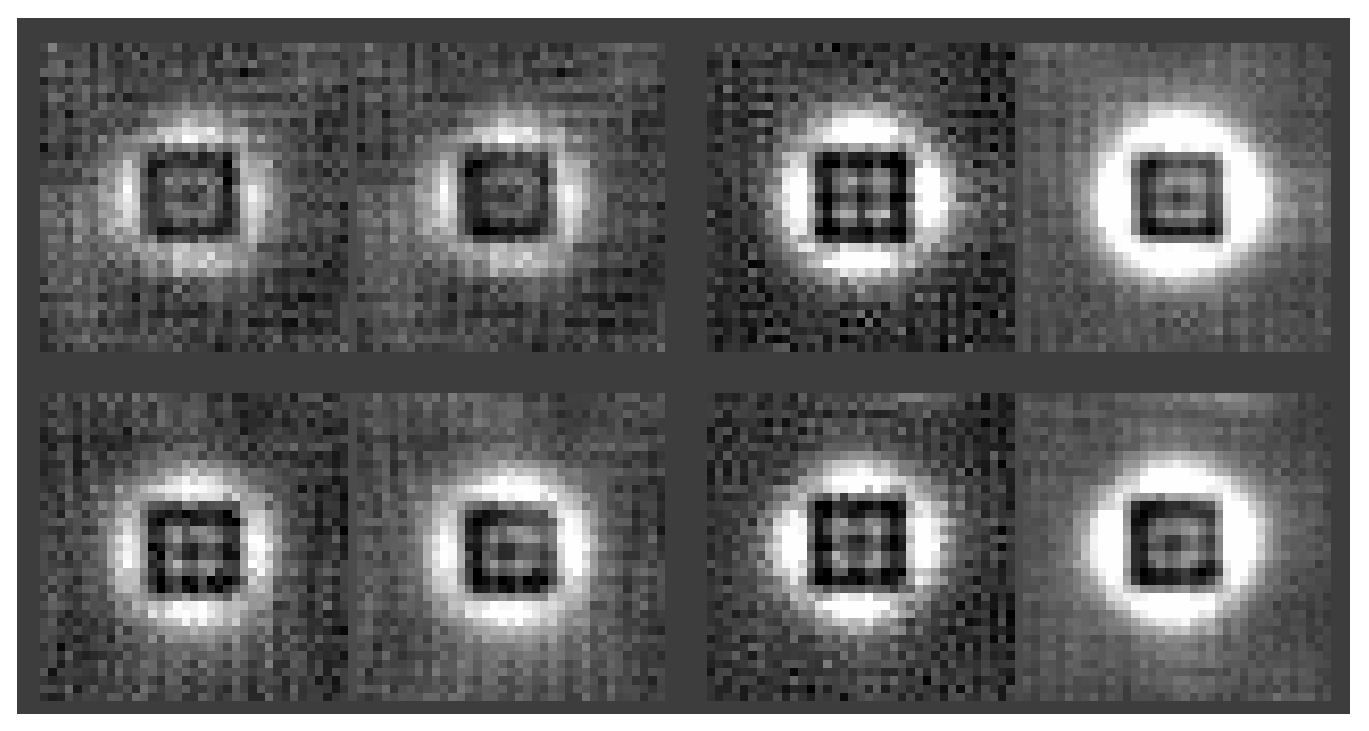
\includegraphics[width=0.5\textwidth, height=0.25\textwidth]{figures/size2.eps} \\
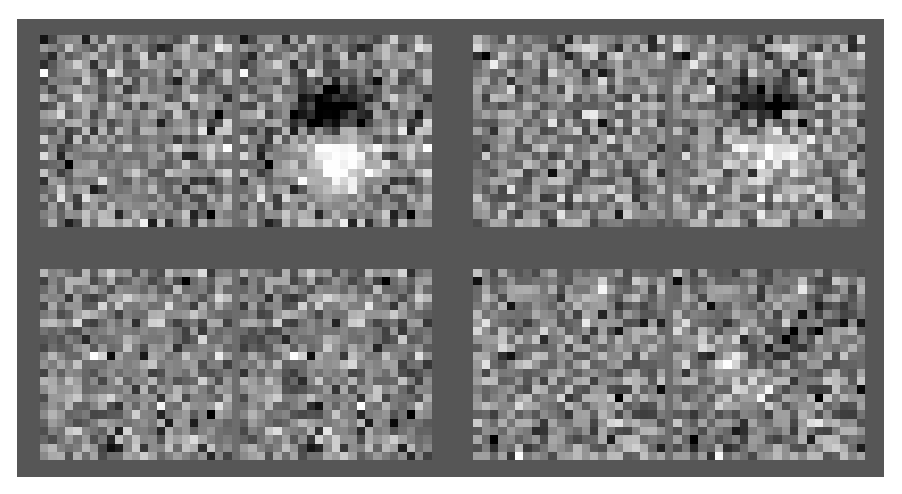
\includegraphics[width=0.5\textwidth, height=0.25\textwidth]{figures/order2.eps} 
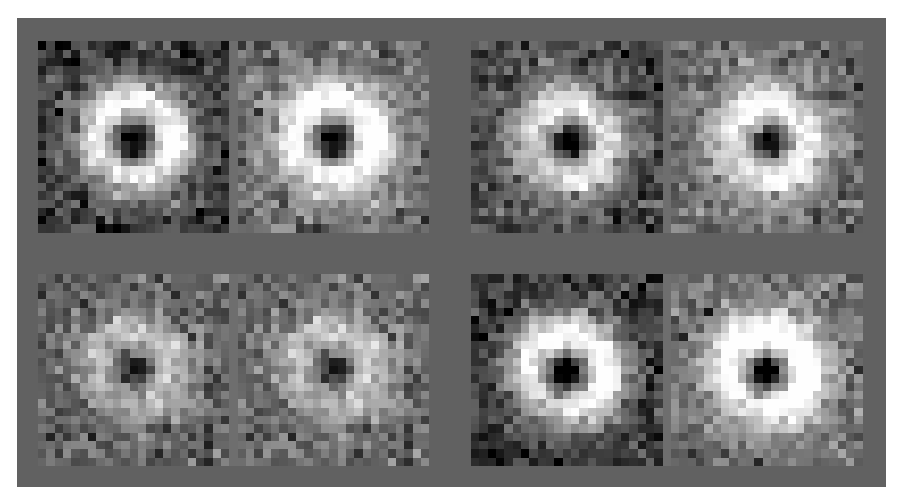
\includegraphics[width=0.5\textwidth, height=0.25\textwidth]{figures/shape2.eps} \\
\caption{Four example panels showing failure modes of the image
  subtraction software.  Each panel itself shows a 2x2 pair of
  difference images; on the {\it left} subpanel is the residual from
  the LOCAL fitting, and on the {\it right} from the SPATIAL fitting.
  Starting in the upper left and going clockwise, the first panel
  shows the residuals when deconvolving the template image; the
  ringing is characteristic of the deconvolution process.  Next, a set
  of difference images where the kernel dimensions (kernelSize) are
  too small to match the sources, leaving square kernel--sized
  residuals around each object.  Next, a set of images where the
  kernel shape (sigGauss) is inappropriate to match the sources; note
  that the LOCAL residuals show circular residuals, indicating the
  basis set itself is at fault (as opposed to the spatial model).
  Finally, in the lower--left, a set of images that demonstrate how
  the residuals degrade when the spatial kernel model is at fault.
  Note that the LOCAL residuals appear to be white noise, while the
  SPATIAL residuals show a clear dipole signature.  For this reason, a
  comparison between the LOCAL and SPATIAL residuals is a useful
  diagnostic of the spatial model.  }
\label{fig_galleryBad}
\end{figure}

\begin{figure}
\begin{center}
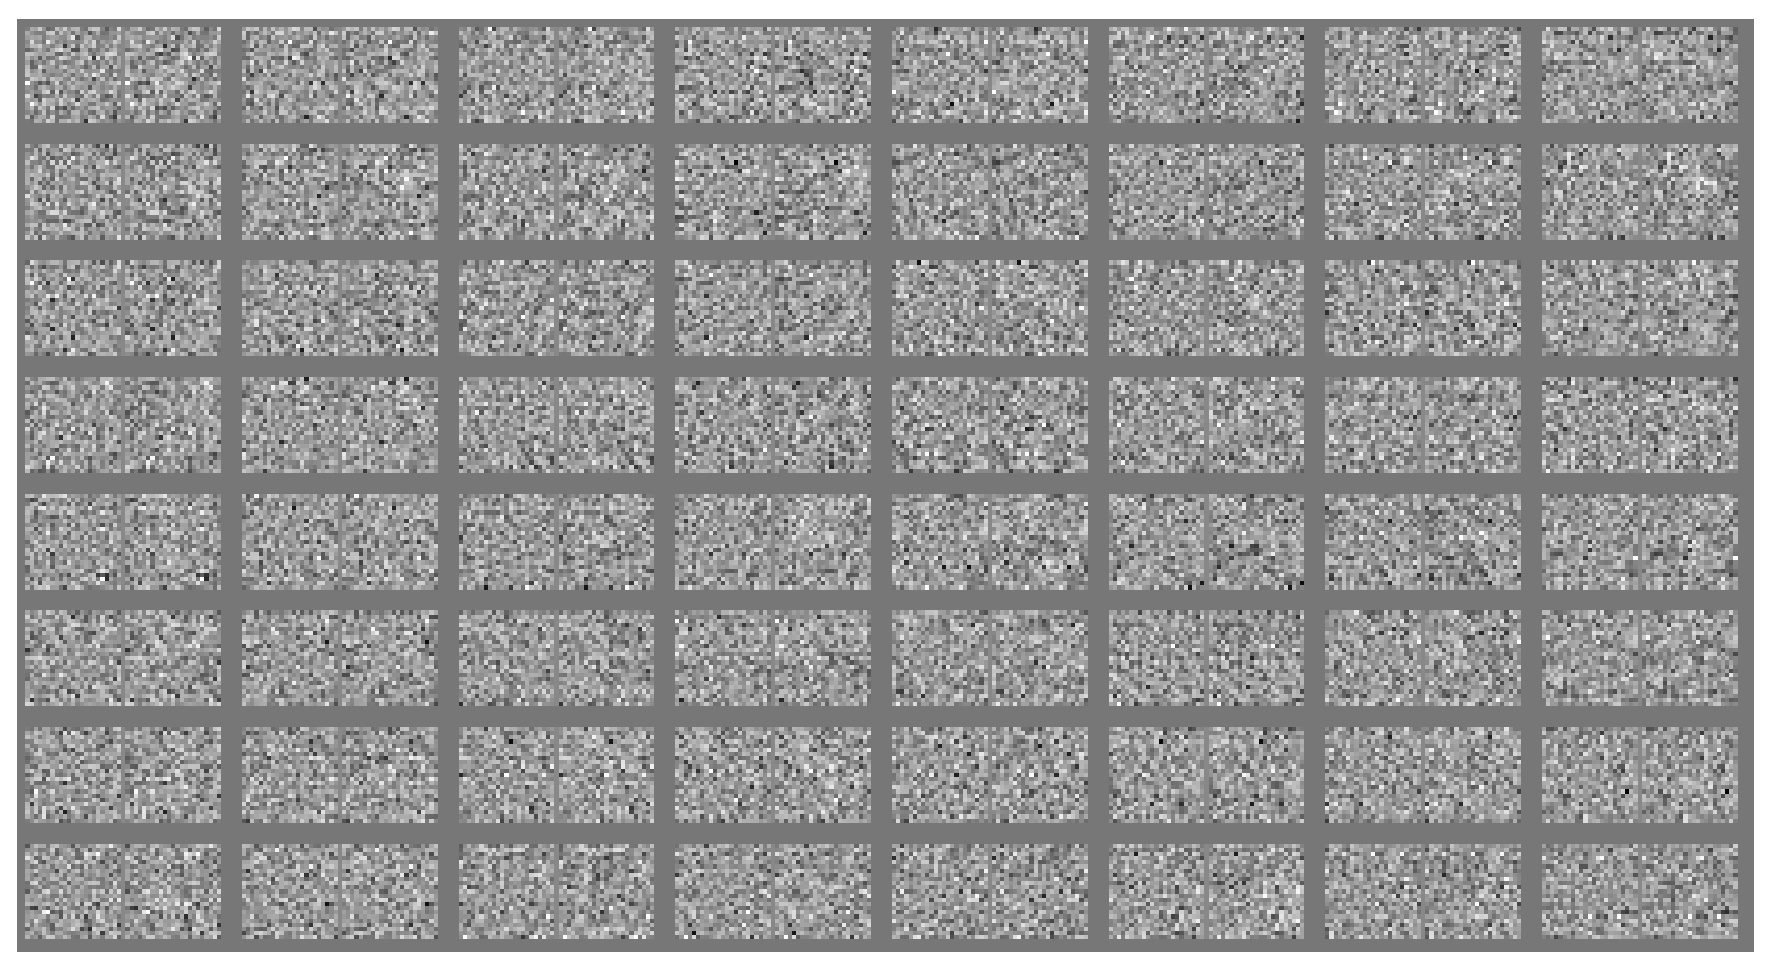
\includegraphics[width=0.9\textwidth]{figures/normal2.eps} \\
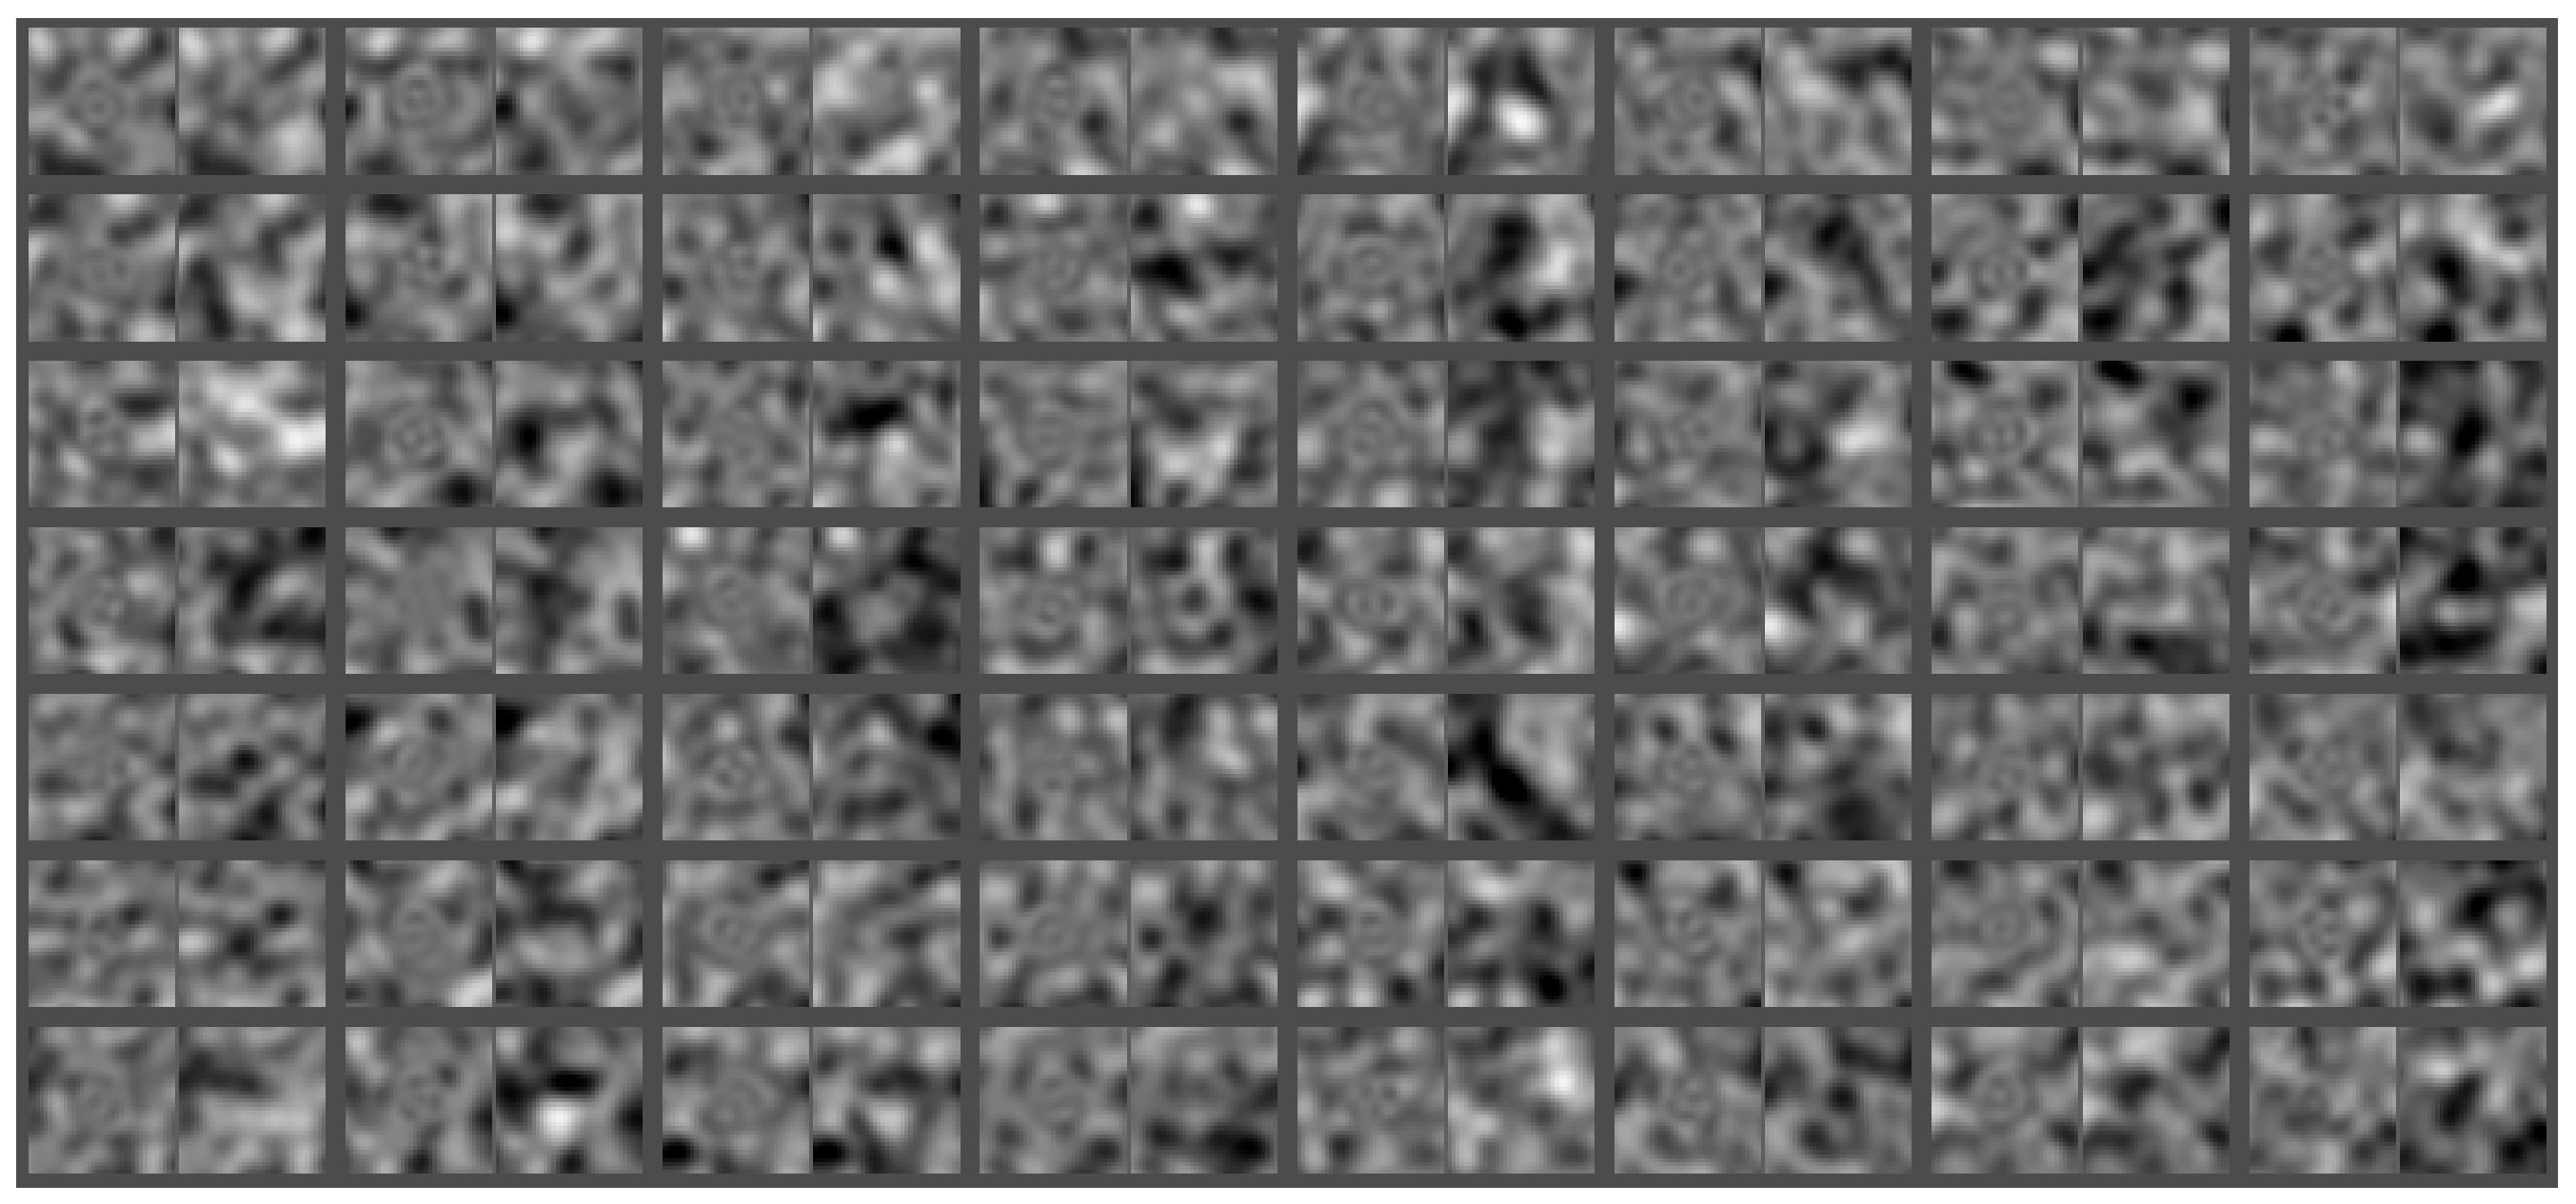
\includegraphics[width=0.9\textwidth]{figures/preconv2.eps} \\
\end{center}
\caption{Pairs of LOCAL,SPATIAL difference images in the case of
  successful image subtraction, similar to
  Figure~\ref{fig_galleryBad}.  The {\it top} set of data are from
  postfiltered analysis, while the {\it lower} set are from
  prefiltered data.  Note that the noise is smoother in the
  prefiltered data due to correlation with the Psf. }
\label{fig_galleryGood}
\end{figure}

\begin{figure}
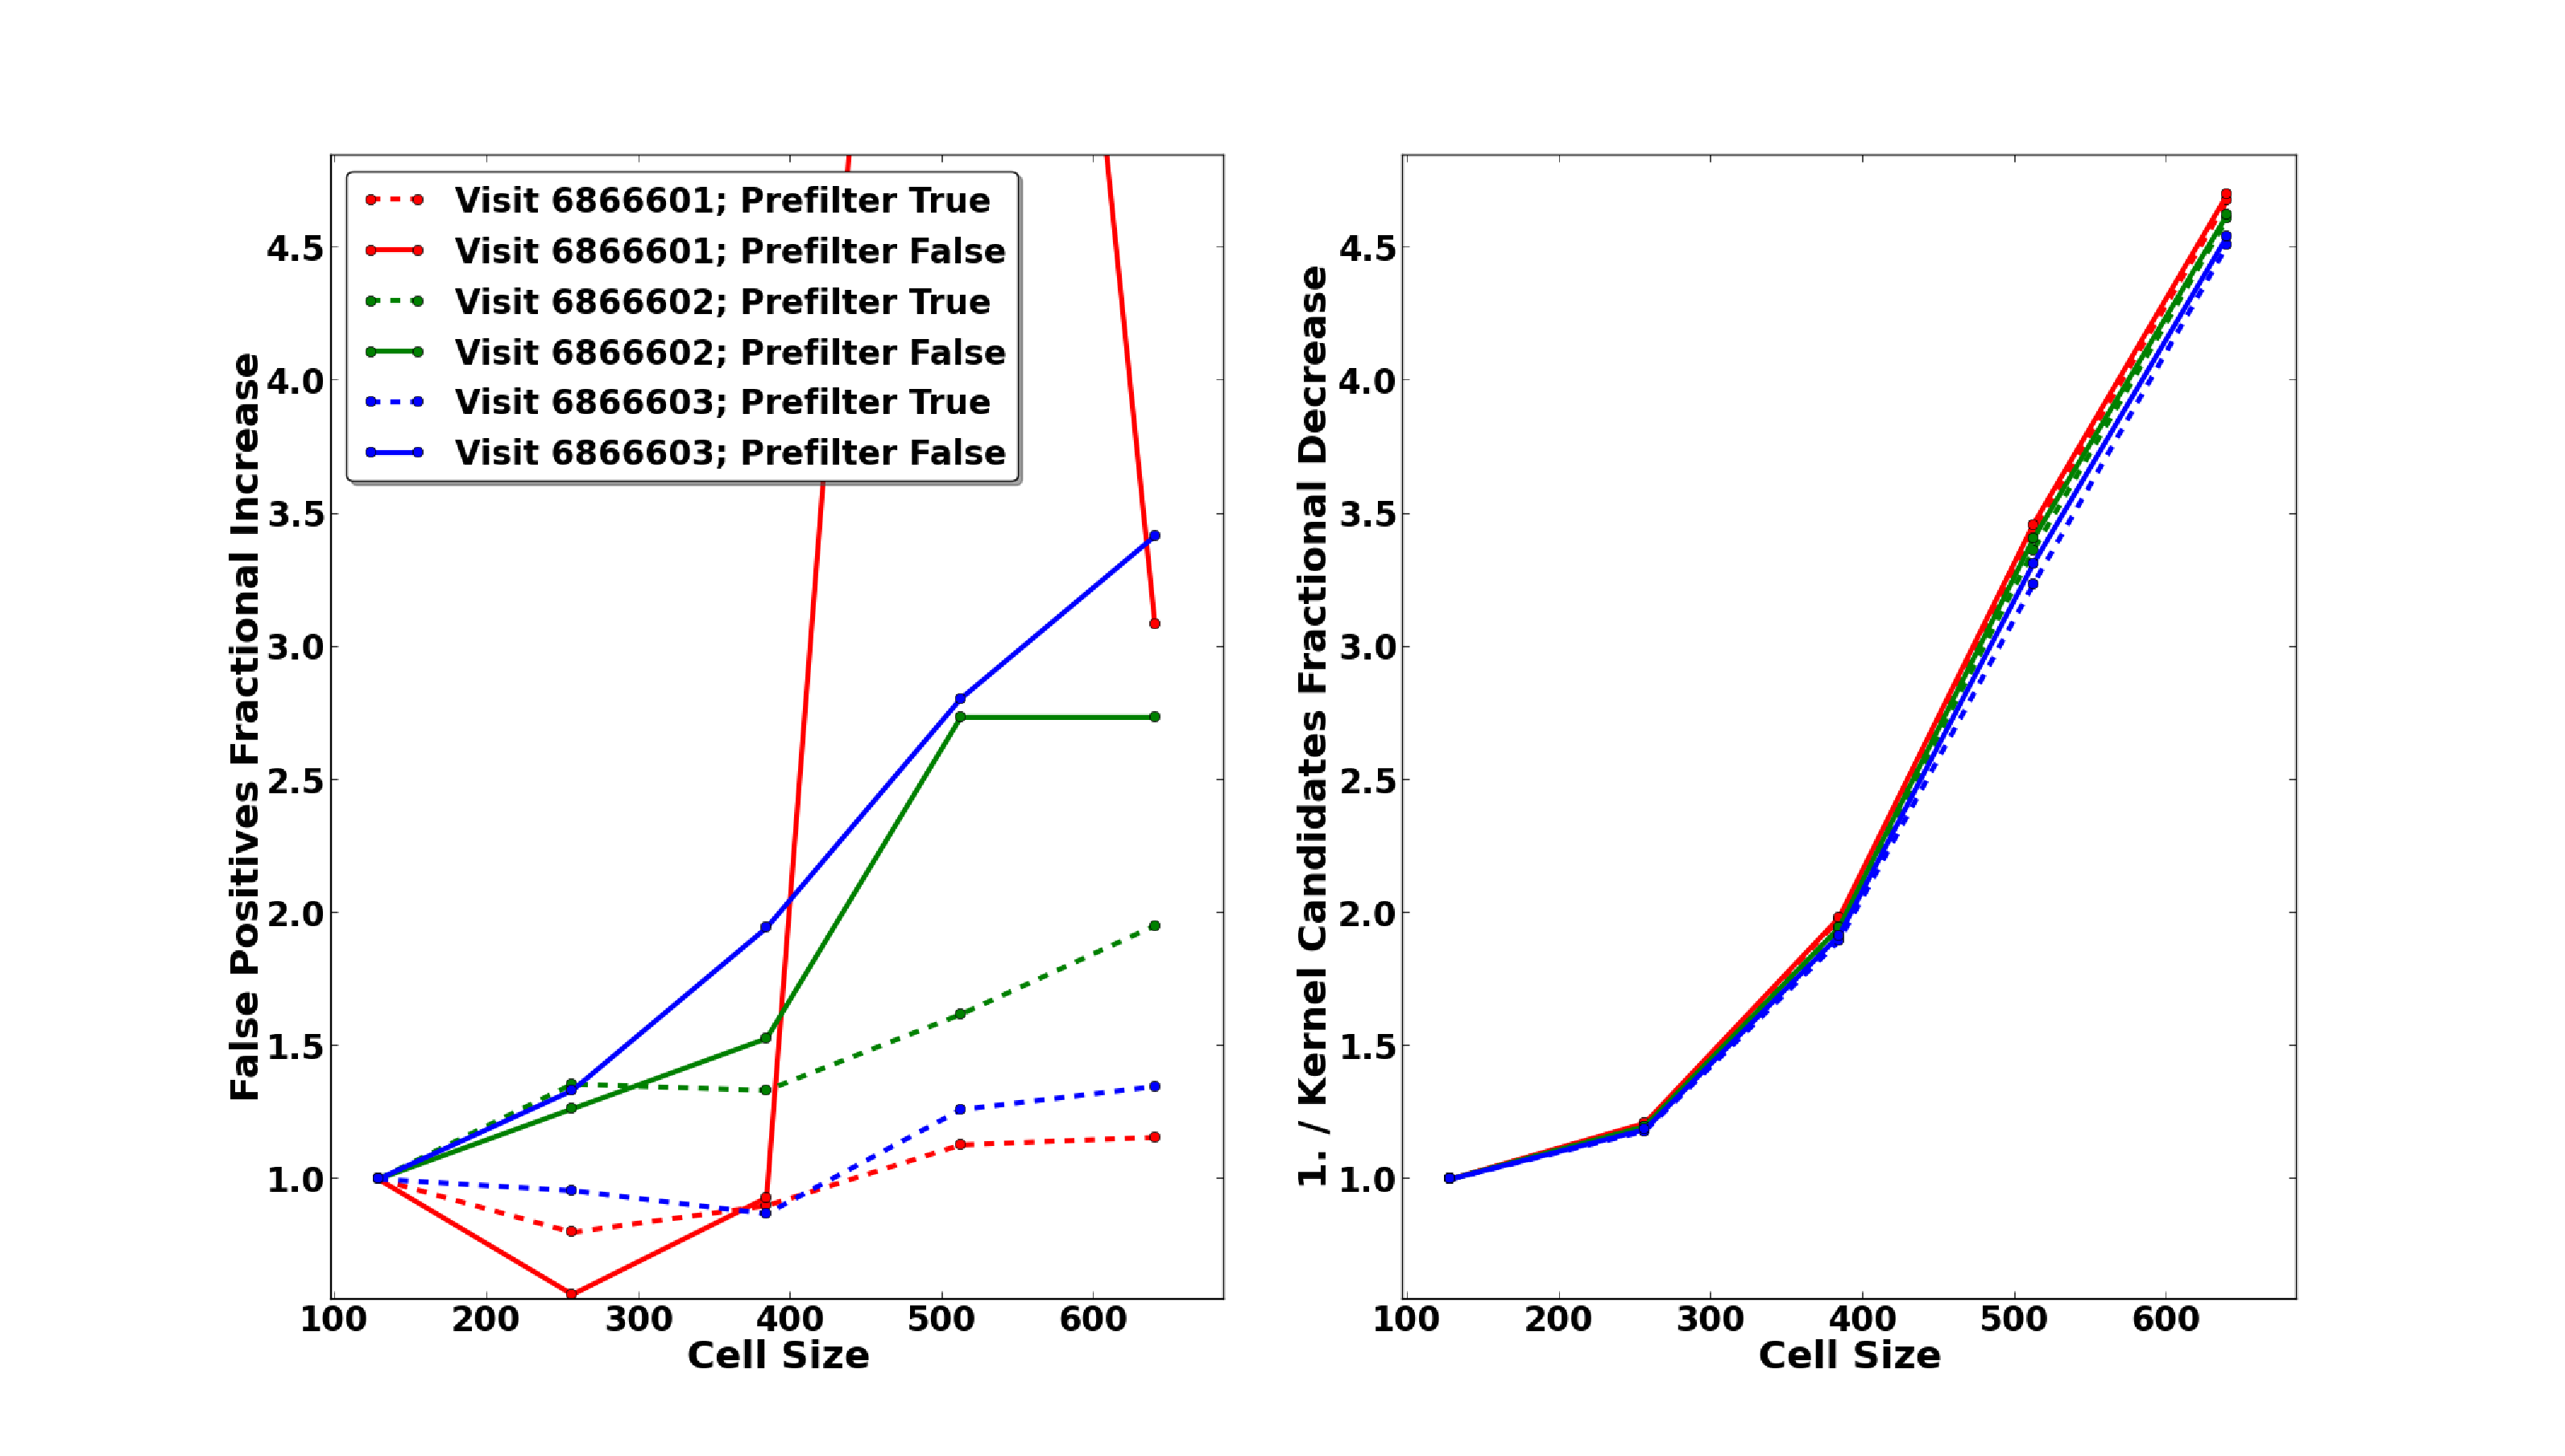
\includegraphics[width=1.0\textwidth]{figures/cellsize.eps} \\
\caption{False detections with cell size
}
\label{cellsize}
\end{figure}

\begin{figure}
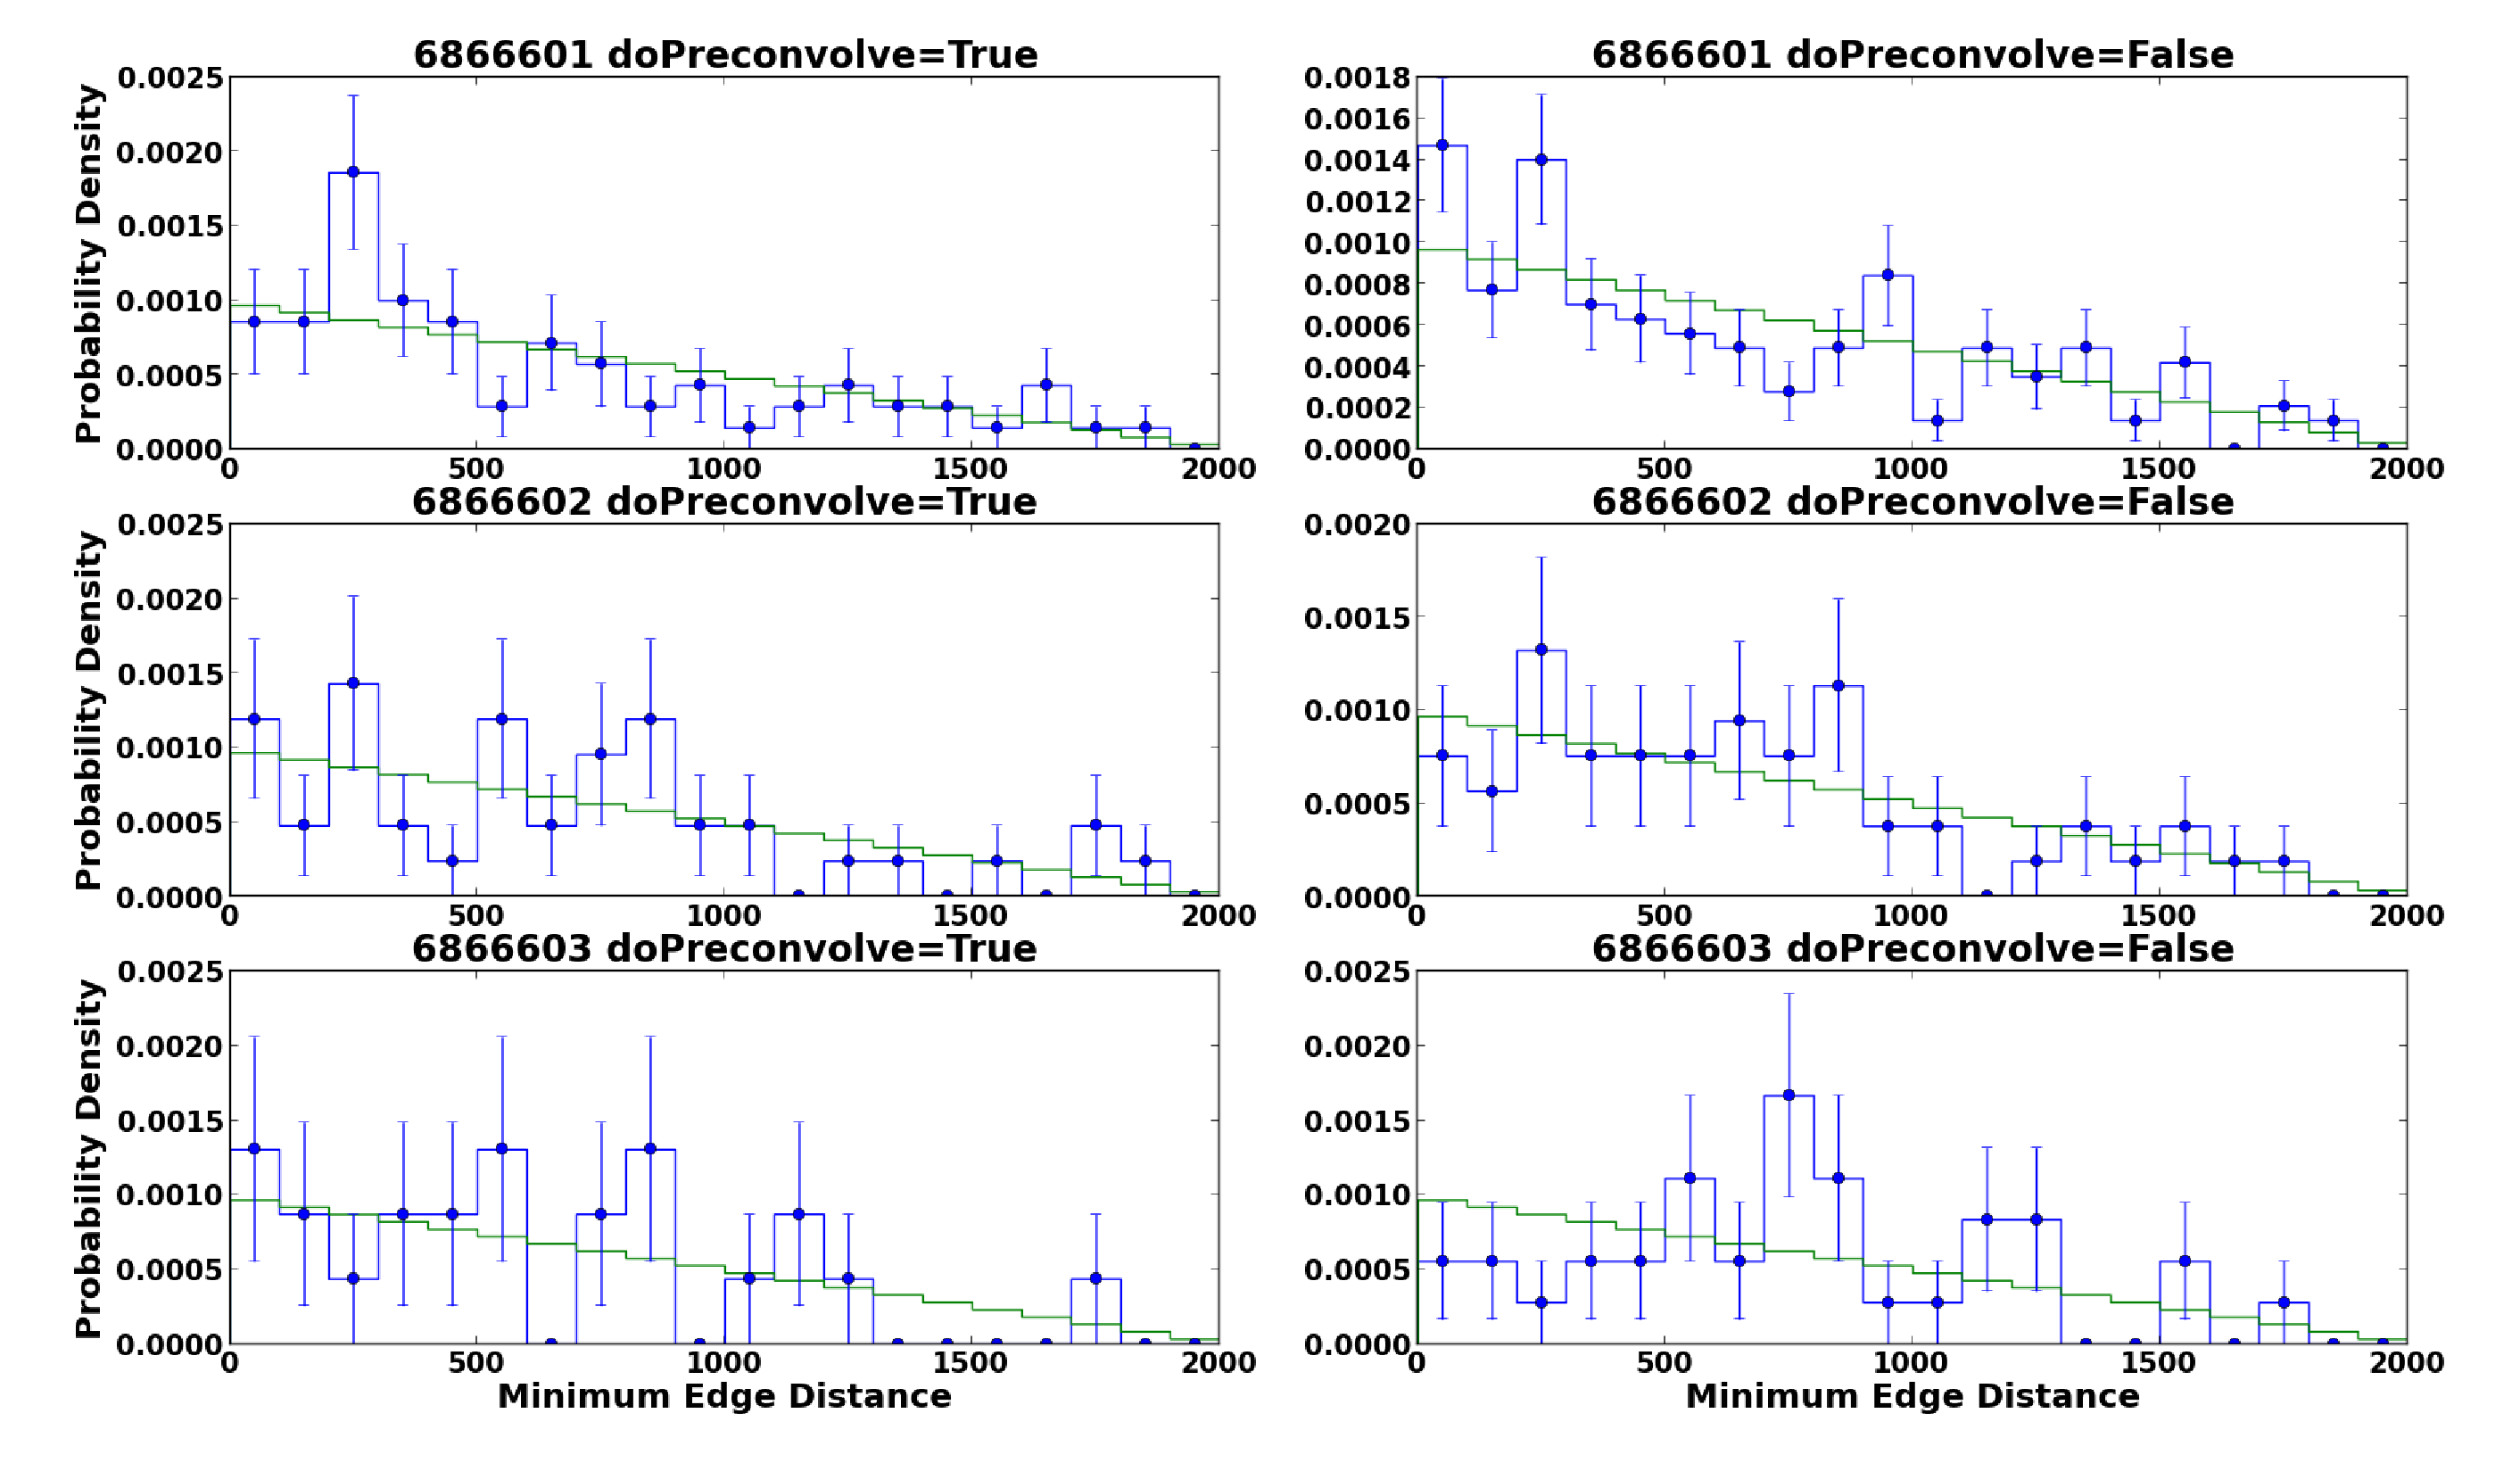
\includegraphics[width=1.0\textwidth]{figures/edge.eps} \\
\caption{Distribution of false detections as a function of the minimum
  distance from the edge of the sensor.  The {\it green} line shows
  the results from a random distribution of points.  The {\it blue}
  lines show the measured distributions, normalized as a probability
  density ($\sum y~\Delta x = 1$).  Error bars come from the square
  root of the number of points in each bin. }
\label{edgedist}
\end{figure}

\begin{figure}
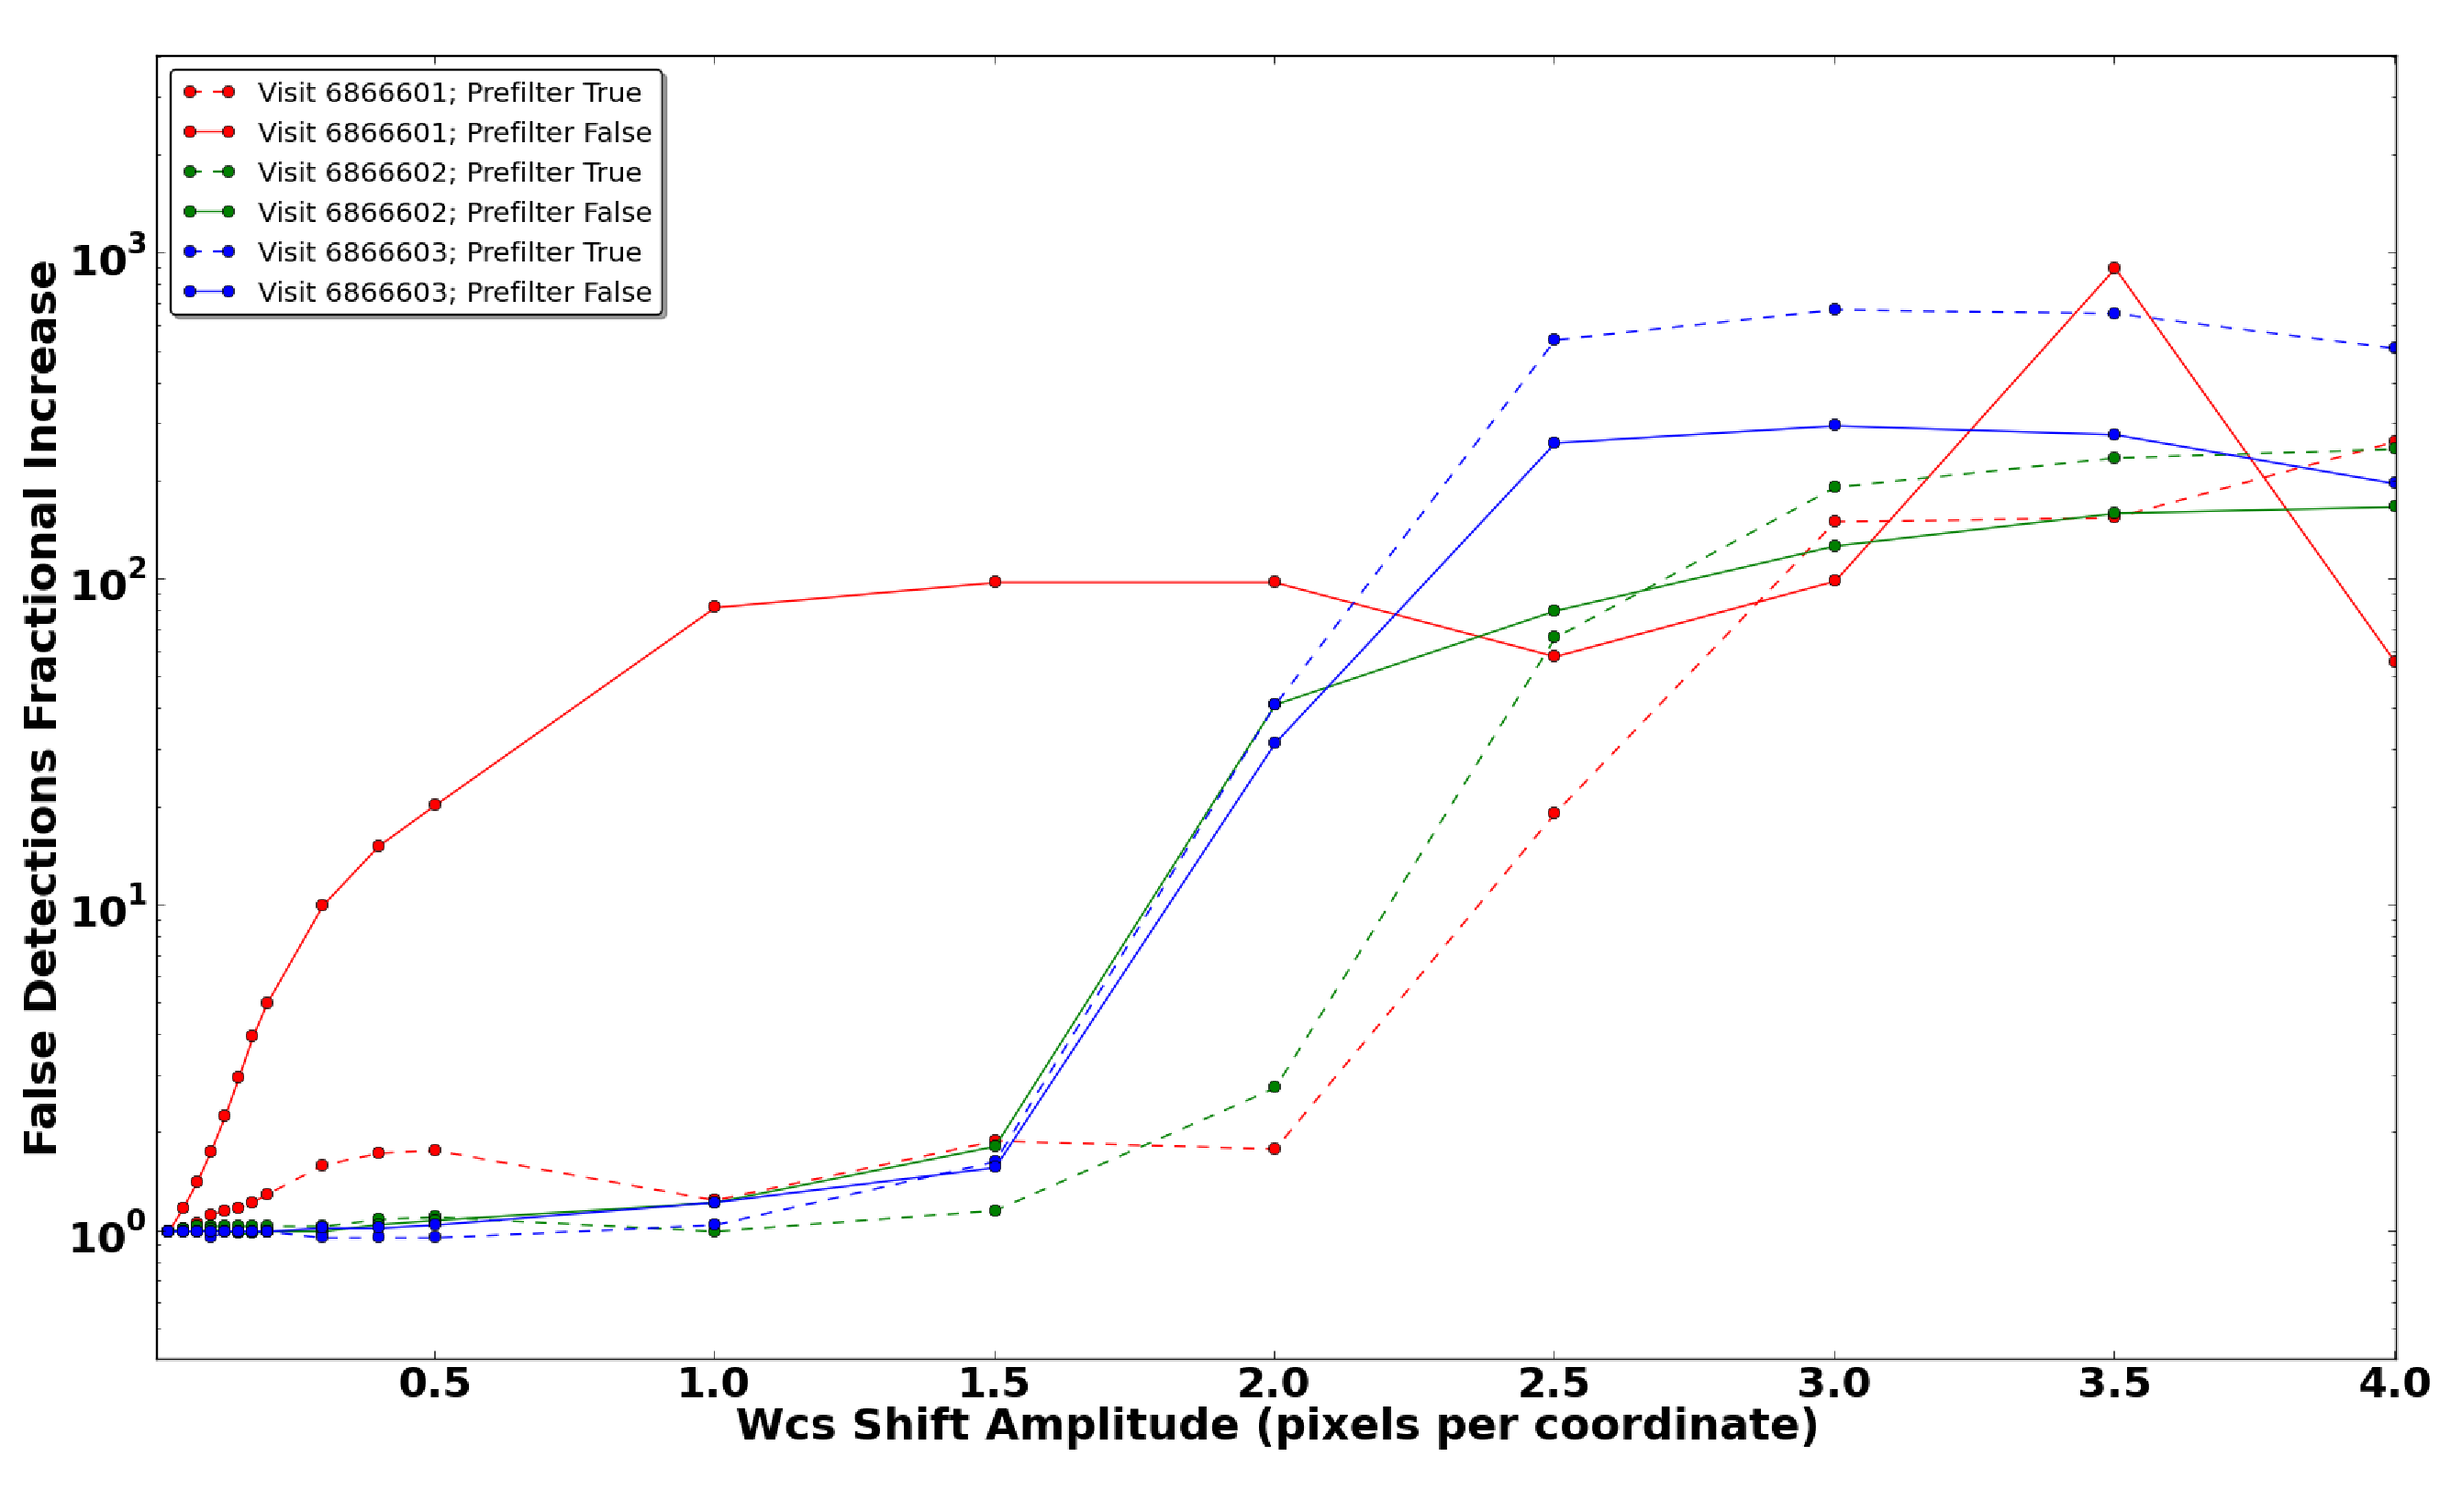
\includegraphics[width=1.0\textwidth]{figures/wcs_shift.eps} \\
\caption{Wcs shift.}
\label{wcsshift}
\end{figure}

\begin{figure}
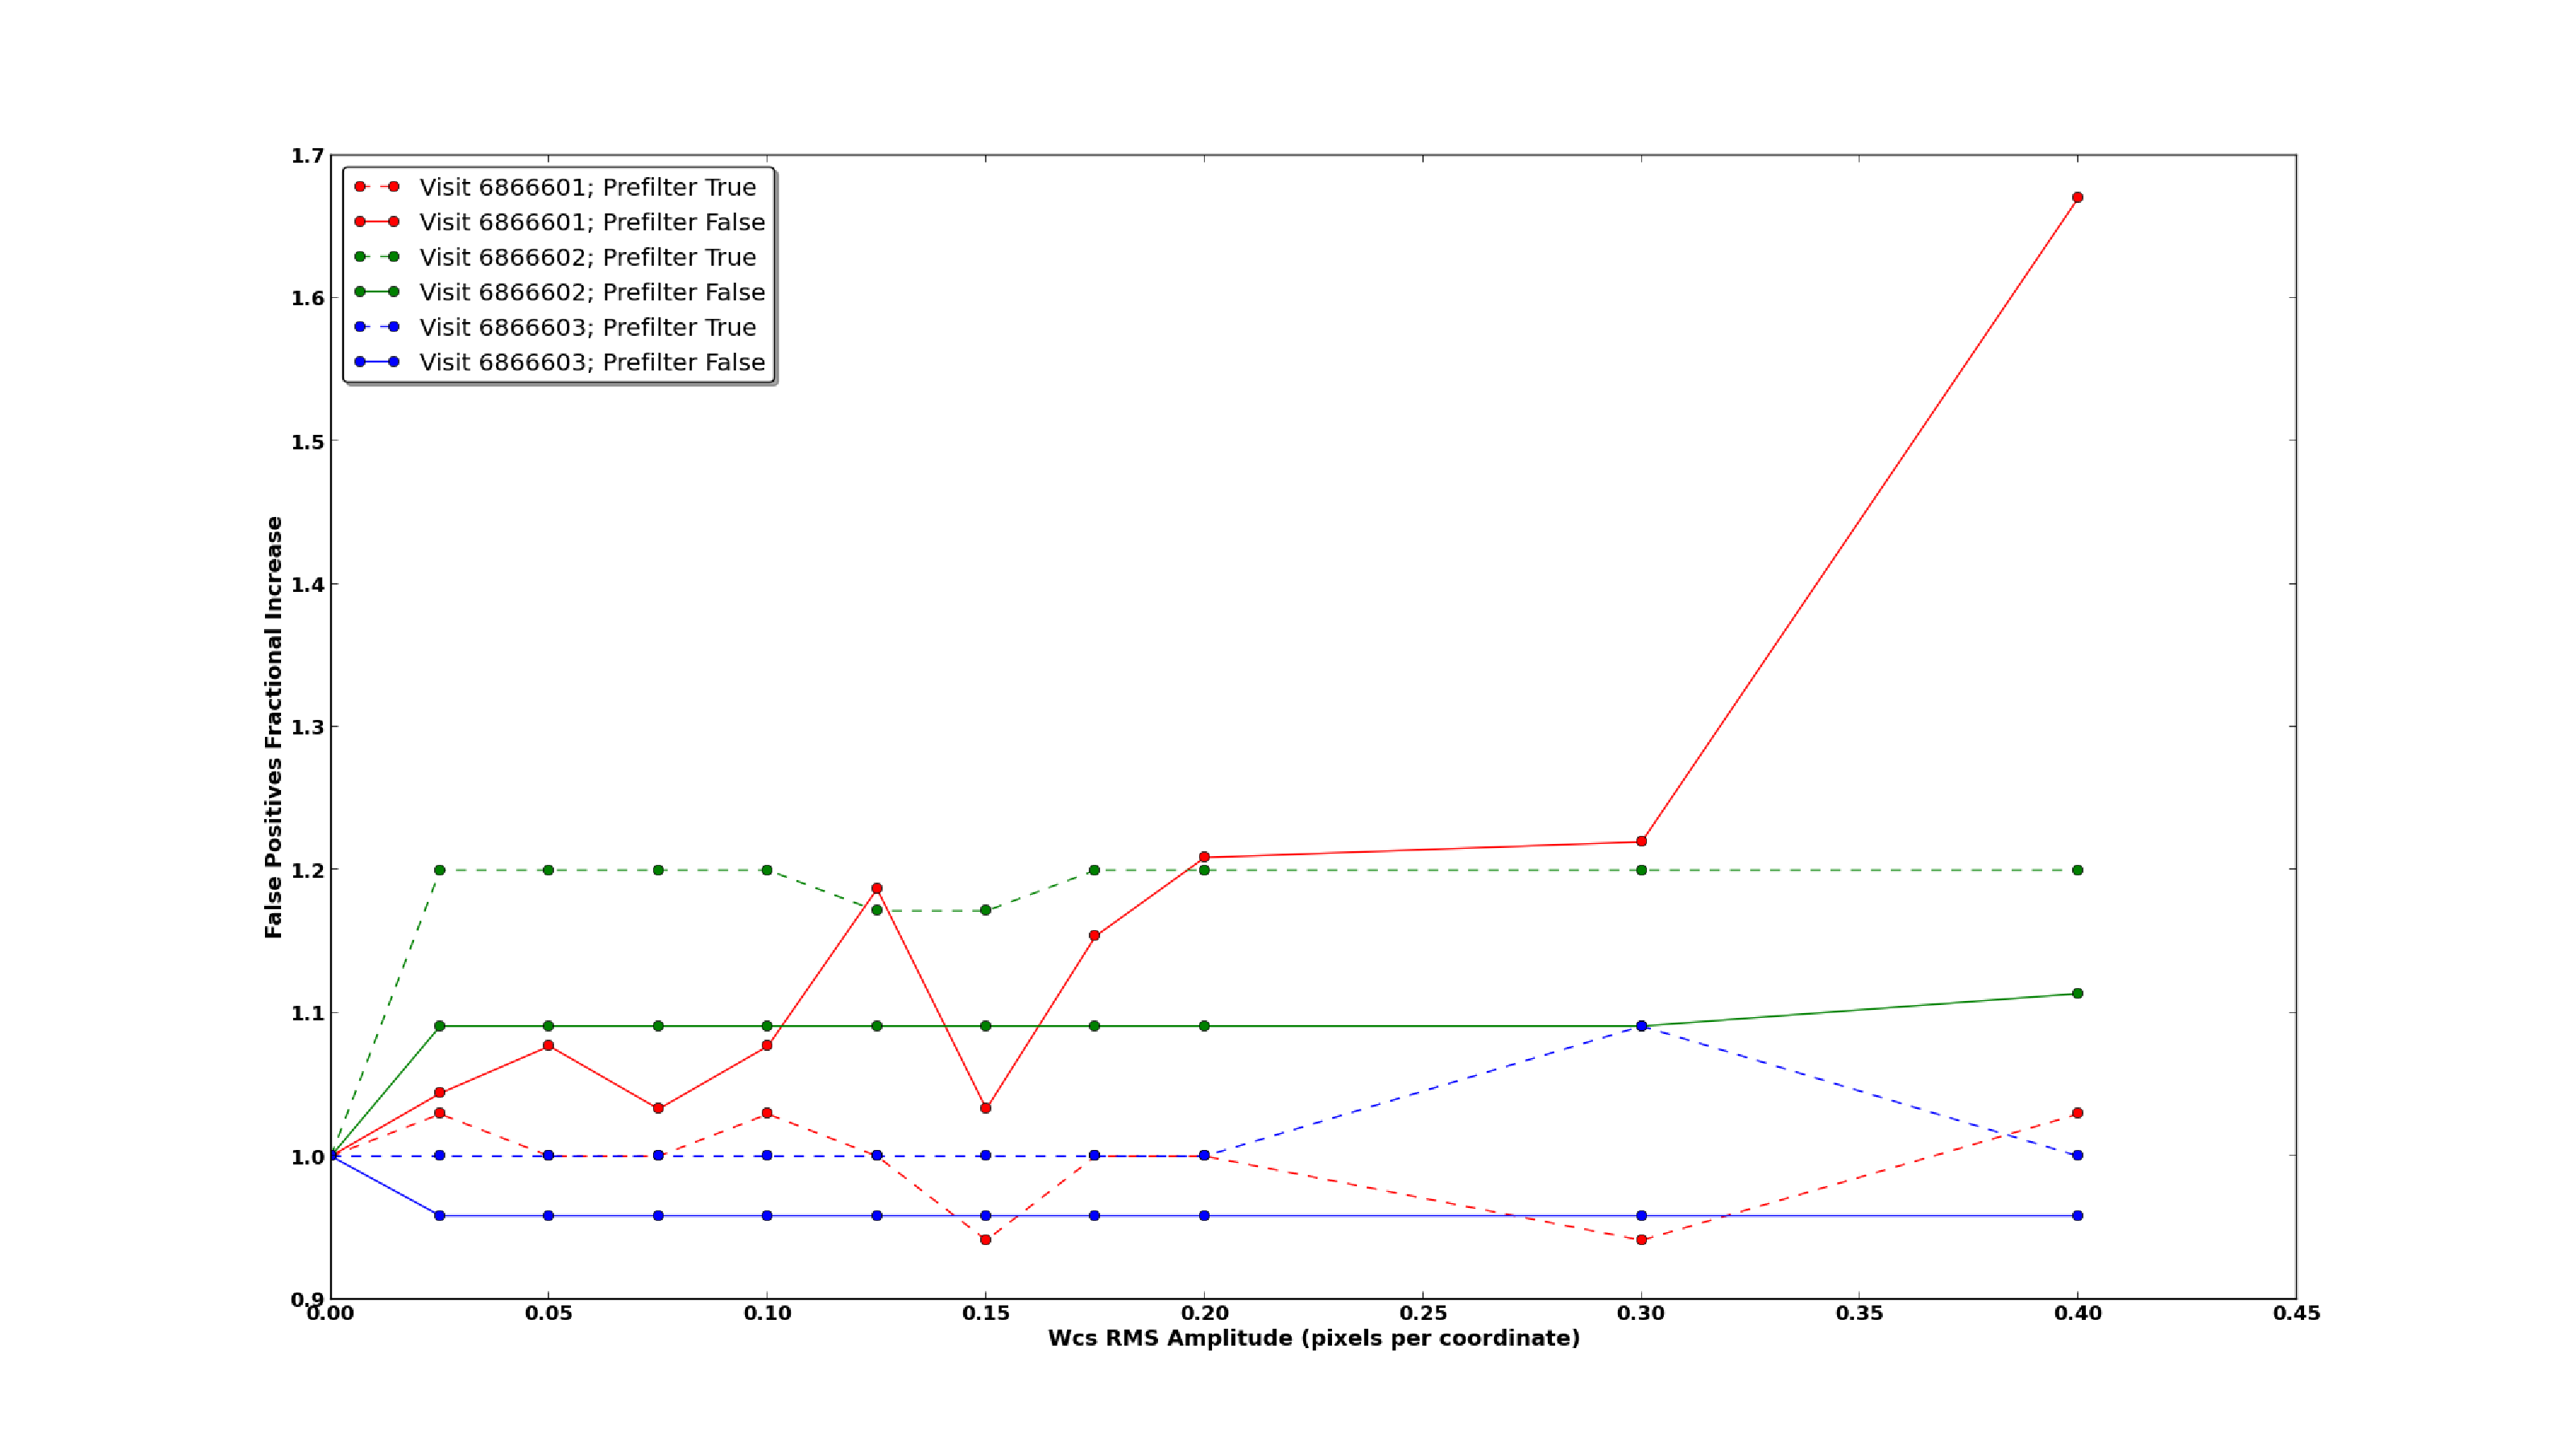
\includegraphics[width=1.0\textwidth]{figures/wcs_rms.eps} \\
\caption{Wcs rms.}
\label{wcsrms}
\end{figure}


\end{document}
